\documentclass[jkps,preprint,fleqn,showpacs,showkeys]{revtex4}
%DIF LATEXDIFF DIFFERENCE FILE
%DIF DEL /Users/junleekim/Downloads/JKPS_KOTO_Emcal_7858/paper.tex   Mon Feb  7 07:31:30 2022
%DIF ADD paper.tex                                                   Mon Feb  7 16:24:33 2022

\usepackage{graphicx}
\usepackage{amssymb}
\usepackage{amsmath}
\usepackage{bm}
\usepackage{lineno}
\usepackage{xspace}
\usepackage{cleveref}
%DIF 10a10
\usepackage{stackengine} %DIF > 
%DIF -------
\usepackage {xcolor}

\newcommand{\XGB}{XGBoost}
%DIF PREAMBLE EXTENSION ADDED BY LATEXDIFF
%DIF UNDERLINE PREAMBLE %DIF PREAMBLE
\RequirePackage[normalem]{ulem} %DIF PREAMBLE
\RequirePackage{color}\definecolor{RED}{rgb}{1,0,0}\definecolor{BLUE}{rgb}{0,0,1} %DIF PREAMBLE
\providecommand{\DIFadd}[1]{{\protect\color{blue}\uwave{#1}}} %DIF PREAMBLE
\providecommand{\DIFdel}[1]{{\protect\color{red}\sout{#1}}}                      %DIF PREAMBLE
%DIF SAFE PREAMBLE %DIF PREAMBLE
\providecommand{\DIFaddbegin}{} %DIF PREAMBLE
\providecommand{\DIFaddend}{} %DIF PREAMBLE
\providecommand{\DIFdelbegin}{} %DIF PREAMBLE
\providecommand{\DIFdelend}{} %DIF PREAMBLE
\providecommand{\DIFmodbegin}{} %DIF PREAMBLE
\providecommand{\DIFmodend}{} %DIF PREAMBLE
%DIF FLOATSAFE PREAMBLE %DIF PREAMBLE
\providecommand{\DIFaddFL}[1]{\DIFadd{#1}} %DIF PREAMBLE
\providecommand{\DIFdelFL}[1]{\DIFdel{#1}} %DIF PREAMBLE
\providecommand{\DIFaddbeginFL}{} %DIF PREAMBLE
\providecommand{\DIFaddendFL}{} %DIF PREAMBLE
\providecommand{\DIFdelbeginFL}{} %DIF PREAMBLE
\providecommand{\DIFdelendFL}{} %DIF PREAMBLE
\newcommand{\DIFscaledelfig}{0.5}
%DIF HIGHLIGHTGRAPHICS PREAMBLE %DIF PREAMBLE
\RequirePackage{settobox} %DIF PREAMBLE
\RequirePackage{letltxmacro} %DIF PREAMBLE
\newsavebox{\DIFdelgraphicsbox} %DIF PREAMBLE
\newlength{\DIFdelgraphicswidth} %DIF PREAMBLE
\newlength{\DIFdelgraphicsheight} %DIF PREAMBLE
% store original definition of \includegraphics %DIF PREAMBLE
\LetLtxMacro{\DIFOincludegraphics}{\includegraphics} %DIF PREAMBLE
\newcommand{\DIFaddincludegraphics}[2][]{{\color{blue}\fbox{\DIFOincludegraphics[#1]{#2}}}} %DIF PREAMBLE
\newcommand{\DIFdelincludegraphics}[2][]{% %DIF PREAMBLE
\sbox{\DIFdelgraphicsbox}{\DIFOincludegraphics[#1]{#2}}% %DIF PREAMBLE
\settoboxwidth{\DIFdelgraphicswidth}{\DIFdelgraphicsbox} %DIF PREAMBLE
\settoboxtotalheight{\DIFdelgraphicsheight}{\DIFdelgraphicsbox} %DIF PREAMBLE
\scalebox{\DIFscaledelfig}{% %DIF PREAMBLE
\parbox[b]{\DIFdelgraphicswidth}{\usebox{\DIFdelgraphicsbox}\\[-\baselineskip] \rule{\DIFdelgraphicswidth}{0em}}\llap{\resizebox{\DIFdelgraphicswidth}{\DIFdelgraphicsheight}{% %DIF PREAMBLE
\setlength{\unitlength}{\DIFdelgraphicswidth}% %DIF PREAMBLE
\begin{picture}(1,1)% %DIF PREAMBLE
\thicklines\linethickness{2pt} %DIF PREAMBLE
{\color[rgb]{1,0,0}\put(0,0){\framebox(1,1){}}}% %DIF PREAMBLE
{\color[rgb]{1,0,0}\put(0,0){\line( 1,1){1}}}% %DIF PREAMBLE
{\color[rgb]{1,0,0}\put(0,1){\line(1,-1){1}}}% %DIF PREAMBLE
\end{picture}% %DIF PREAMBLE
}\hspace*{3pt}}} %DIF PREAMBLE
} %DIF PREAMBLE
\LetLtxMacro{\DIFOaddbegin}{\DIFaddbegin} %DIF PREAMBLE
\LetLtxMacro{\DIFOaddend}{\DIFaddend} %DIF PREAMBLE
\LetLtxMacro{\DIFOdelbegin}{\DIFdelbegin} %DIF PREAMBLE
\LetLtxMacro{\DIFOdelend}{\DIFdelend} %DIF PREAMBLE
\DeclareRobustCommand{\DIFaddbegin}{\DIFOaddbegin \let\includegraphics\DIFaddincludegraphics} %DIF PREAMBLE
\DeclareRobustCommand{\DIFaddend}{\DIFOaddend \let\includegraphics\DIFOincludegraphics} %DIF PREAMBLE
\DeclareRobustCommand{\DIFdelbegin}{\DIFOdelbegin \let\includegraphics\DIFdelincludegraphics} %DIF PREAMBLE
\DeclareRobustCommand{\DIFdelend}{\DIFOaddend \let\includegraphics\DIFOincludegraphics} %DIF PREAMBLE
\LetLtxMacro{\DIFOaddbeginFL}{\DIFaddbeginFL} %DIF PREAMBLE
\LetLtxMacro{\DIFOaddendFL}{\DIFaddendFL} %DIF PREAMBLE
\LetLtxMacro{\DIFOdelbeginFL}{\DIFdelbeginFL} %DIF PREAMBLE
\LetLtxMacro{\DIFOdelendFL}{\DIFdelendFL} %DIF PREAMBLE
\DeclareRobustCommand{\DIFaddbeginFL}{\DIFOaddbeginFL \let\includegraphics\DIFaddincludegraphics} %DIF PREAMBLE
\DeclareRobustCommand{\DIFaddendFL}{\DIFOaddendFL \let\includegraphics\DIFOincludegraphics} %DIF PREAMBLE
\DeclareRobustCommand{\DIFdelbeginFL}{\DIFOdelbeginFL \let\includegraphics\DIFdelincludegraphics} %DIF PREAMBLE
\DeclareRobustCommand{\DIFdelendFL}{\DIFOaddendFL \let\includegraphics\DIFOincludegraphics} %DIF PREAMBLE
%DIF LISTINGS PREAMBLE %DIF PREAMBLE
\RequirePackage{listings} %DIF PREAMBLE
\RequirePackage{color} %DIF PREAMBLE
\lstdefinelanguage{DIFcode}{ %DIF PREAMBLE
%DIF DIFCODE_UNDERLINE %DIF PREAMBLE
  moredelim=[il][\color{red}\sout]{\%DIF\ <\ }, %DIF PREAMBLE
  moredelim=[il][\color{blue}\uwave]{\%DIF\ >\ } %DIF PREAMBLE
} %DIF PREAMBLE
\lstdefinestyle{DIFverbatimstyle}{ %DIF PREAMBLE
	language=DIFcode, %DIF PREAMBLE
	basicstyle=\ttfamily, %DIF PREAMBLE
	columns=fullflexible, %DIF PREAMBLE
	keepspaces=true %DIF PREAMBLE
} %DIF PREAMBLE
\lstnewenvironment{DIFverbatim}{\lstset{style=DIFverbatimstyle}}{} %DIF PREAMBLE
\lstnewenvironment{DIFverbatim*}{\lstset{style=DIFverbatimstyle,showspaces=true}}{} %DIF PREAMBLE
%DIF END PREAMBLE EXTENSION ADDED BY LATEXDIFF

\begin{document}
\setcounter{page}{0}
\title[]{\DIFdelbegin \DIFdel{MC-based feasibility study }\DIFdelend \DIFaddbegin \DIFadd{Simulation Study }\DIFaddend of \DIFdelbegin \DIFdel{new sampling calorimeter for measuring the $\gamma$ incident angle }\DIFdelend \DIFaddbegin \DIFadd{Angular Resolution of a New Electromagnetic Sampling Calorimeter}\DIFaddend }

\author{YoungJun \surname{Kim}}
\author{Jung Keun \surname{Ahn}}
\affiliation{Department of Physics, Korea University, Seoul 02841}
\author{Junlee \surname{Kim}}
\email{junlee.kim@cern.ch}
\author{Eun-Joo \surname{Kim}}
\email{ejkim@jbnu.ac.kr}
\affiliation{Department of Physics education, Jeonbuk National University, Jeonju 54896}
\author{GeiYoub  \surname{Lim}}
\affiliation{IPNS/KEK Tsukuba, Japan 305-0801}

%\date[]{Received 6 August 2007}

\begin{abstract}
We \DIFdelbegin \DIFdel{present studies on the detector configuration to measure the incident angle of the $\gamma$ with energies ranging from hundred MeV to few GeVusing a new sampling calorimeter. The sampling }\DIFdelend \DIFaddbegin \DIFadd{report simulation results on the angular resolution of electromagnetic (EM) sampling calorimeters with photons being in the range of 100~MeV to 2~GeV. A simulation model of the EM }\DIFaddend calorimeter consists of alternating \DIFaddbegin \DIFadd{layers of a }\DIFaddend 1-mm-thick \DIFdelbegin \DIFdel{lead plates producing the electromagnetic (EM) shower and strips of }\DIFdelend \DIFaddbegin \DIFadd{Pb plate and a }\DIFaddend 5-mm-thick plastic \DIFdelbegin \DIFdel{scintillators measuring the energy deposit by the shower particles. The strips are arranged along the alternating }\DIFdelend \DIFaddbegin \DIFadd{scintillator plate. The scintillator plates are alternatively segmented in }\DIFaddend horizontal and vertical \DIFdelbegin \DIFdel{directions to measure the transverse profile by combining both directions at a given longitudinal position}\DIFdelend \DIFaddbegin \DIFadd{strips}\DIFaddend . In this \DIFdelbegin \DIFdel{paper, we used the GEANT4 to simulate energy deposit to the individual strips of the calorimeter, and the $\XGB$ to reconstruct the incident angle from energy deposits. }%DIFDELCMD < 

%DIFDELCMD < %%%
\DIFdel{The angular resolution weakly depends on the width of the strips up to 15 mm and becomes worse with the increasing width. It is found that the incident angle is reconstructed with the compatible angular resolution using front 5 radiation length }\DIFdelend \DIFaddbegin \DIFadd{study, we obtained energy deposit in individual strips using Geant4 simulations and reconstructed incident photon angles using a XGBoost model with boosted decision trees. Angular resolutions are studied in terms of the strip width. The 15-mm-wide strips provide the best angular resolution of 1.23~$\pm$~0.01$^{\circ}$. Incident photon directions can be well reconstructed in the front part }\DIFaddend (5$X_{0}$) of the \DIFdelbegin \DIFdel{detector. The resolution does not depend on the incident angle up to }\DIFdelend \DIFaddbegin \DIFadd{EM calorimeter. The angular resolution is almost constant for small angles less than }\DIFaddend 30\DIFdelbegin \DIFdel{degrees, and largely depends on the incident energy, which }\DIFdelend \DIFaddbegin \DIFadd{$^{\circ}$, and varies significantly with the incident photon energy. The
energy dependence }\DIFaddend can be expressed as \DIFdelbegin \DIFdel{0.2+1.1$/ \sqrt{E_\gamma}$}\DIFdelend \DIFaddbegin \DIFadd{$\sigma_{\theta}=$~xxx~$\oplus$~yyy~$/\sqrt{E_{\gamma}}$}\DIFaddend .

\end{abstract}

%\pacs{68.37.Ef, 82.20.-w, 68.43.-h}
%DIF < \keywords{String shoving, Collectivity, $pp$ collision}
\DIFaddbegin \keywords{Electromagnetic Calorimeter, Geant4, XGBoost, KOTO}
\DIFaddend \maketitle

\section{Motivation}
\label{sec:mot}
The \DIFdelbegin \DIFdel{EM calorimeter has played }\DIFdelend \DIFaddbegin \DIFadd{electromagnetic (EM) calorimeter plays }\DIFaddend an important role in experimental studies for the nuclear and particle physics. Various materials have been developed for better energy and timing \DIFdelbegin \DIFdel{resolution }\DIFdelend \DIFaddbegin \DIFadd{resolutions }\DIFaddend so far~\cite{Calorimeter}. \DIFaddbegin \DIFadd{EM calorimeters can be divided into two groups: sampling calorimeters and homogeneous calorimeter. Sampling calorimeters consist of alternating layers of an absorber generating EM showers and an active medium providing signals. }\DIFaddend On the other \DIFdelbegin \DIFdel{side, }\DIFdelend \DIFaddbegin \DIFadd{hand, homogeneous calorimeters are built of only a single type of material that facilitates both EM showers and signal generations. Today, }\DIFaddend the sampling calorimeter becomes \DIFdelbegin \DIFdel{popular in the }\DIFdelend \DIFaddbegin \DIFadd{very popular in }\DIFaddend large-scale high energy \DIFdelbegin \DIFdel{experiment mainly due }\DIFdelend \DIFaddbegin \DIFadd{experiments, owing }\DIFaddend to its cost-effectiveness. \DIFdelbegin \DIFdel{The sampling calorimeter consists of alternating passive converters that generate the EM shower and active counters that measure the energy deposit. Since the energy deposit in the passive convert is not measured, the fluctuation of energy deposits in the converter and the counter, called sampling fluctuation , determines }\DIFdelend \DIFaddbegin \DIFadd{In sampling calorimeters the energy deposited in the active medium fluctuates because the active layers are interleaved with absorber layers. This so-called sampling fluctuation dominates }\DIFaddend the energy resolution\DIFdelbegin \DIFdel{of the calorimeter.
}\DIFdelend \DIFaddbegin \DIFadd{.
}

\DIFaddend The sampling fluctuation can be \DIFdelbegin \DIFdel{optimized by combining the converter and the counter with a specific portion. A 5-m-long }\DIFdelend \DIFaddbegin \DIFadd{improved by optimizing the thickness ratio of the absorber to the active medium. A 3-m-long }\DIFaddend cylindrical calorimeter made of alternating \DIFdelbegin \DIFdel{lead plates }\DIFdelend \DIFaddbegin \DIFadd{layers of Pb }\DIFaddend and plastic scintillating plates is an example of the sampling calorimeter~\DIFdelbegin \DIFdel{\mbox{%DIFAUXCMD
\cite{E391a_barrel}}\hspace{0pt}%DIFAUXCMD
}\DIFdelend \DIFaddbegin \DIFadd{\mbox{%DIFAUXCMD
\cite{Murayama:2020mcp}}\hspace{0pt}%DIFAUXCMD
}\DIFaddend .

The \DIFdelbegin \DIFdel{layer }\DIFdelend \DIFaddbegin \DIFadd{segmented }\DIFaddend structure of the \DIFdelbegin \DIFdel{sampling calorimeter allow one to measure the individual profile of the }\DIFdelend \DIFaddbegin \DIFadd{active medium facilitates the measurement of lateral distributions of the EM }\DIFaddend shower along the \DIFdelbegin \DIFdel{beam direction, and the incident angle can be estimated by correlating energy deposits on neighboring layers}\DIFdelend \DIFaddbegin \DIFadd{incident photon direction. The photon direction can also be deduced from the information on the EM shower shape}\DIFaddend . The measurement of \DIFdelbegin \DIFdel{the incident angle largely benefits the background rejection. Of particular, The incident angle will be an important tool for the }\DIFdelend \DIFaddbegin \DIFadd{photon directions can help predict photon production vertices, which is crucial for the background suppression in }\DIFaddend KOTO experiment~\DIFdelbegin \DIFdel{\mbox{%DIFAUXCMD
\cite{KOTOproposal}}\hspace{0pt}%DIFAUXCMD
}\DIFdelend \DIFaddbegin \DIFadd{\mbox{%DIFAUXCMD
\cite{KOTO:2012}}\hspace{0pt}%DIFAUXCMD
}\DIFaddend .

\DIFdelbegin \DIFdel{Since }\DIFdelend \DIFaddbegin \DIFadd{Stochastic behaviors of }\DIFaddend the EM shower \DIFdelbegin \DIFdel{is evolving via stochastic processes, the incident angle would be reconstructed with a certain angular resolution }\DIFdelend \DIFaddbegin \DIFadd{development limit to the angular resolution of the photon direction measurement}\DIFaddend . Energy deposits \DIFdelbegin \DIFdel{from random processes are used to reconstruct the incident angle with the machine learning, which provides better angular resolution. The evolution of the EM shower is generated with the GEANT4, and the $\XGB$ was used }\DIFdelend \DIFaddbegin \DIFadd{in each active layer of a sampling calorimeter fluctuate event by event so that the reconstruction of photon directions necessitates the longitudinal and lateral segmentation of the calorimeter.
}

\DIFadd{This paper describes a machine learning approach based on XGBoost (XGB) model~\mbox{%DIFAUXCMD
\cite{xgboost:2016} }\hspace{0pt}%DIFAUXCMD
with boosted decision trees in order }\DIFaddend to reconstruct the \DIFdelbegin \DIFdel{incident angle.
}%DIFDELCMD < 

%DIFDELCMD < %%%
\DIFdel{In sec~\ref{sec:ems}, generic explanation of the EM shower and its evolution are described. We describe the reconstruction and }\DIFdelend \DIFaddbegin \DIFadd{directions of incident photons entering a sampling calorimeter with alternating layers of a Pb plate and plastic scintillator strips in horizontal and vertical directions. We generated EM showers in a sampling calorimeter using Geant4 simulations. We report on the detector configuration providing the acceptable angular resolution, and report on the }\DIFaddend angular resolution of the \DIFaddbegin \DIFadd{EM }\DIFaddend sampling calorimeter in \DIFdelbegin \DIFdel{sec~\ref{sec:res}. We summarize the study in sec~\ref{sec:sum}}\DIFdelend \DIFaddbegin \DIFadd{terms of the incident angle and energy}\DIFaddend .

\section{\DIFdelbegin \DIFdel{ELECTROMAGNETIC SHOWER}\DIFdelend \DIFaddbegin \DIFadd{Electromagnetic Shower Simulation}\DIFaddend }
\label{sec:ems}

\begin{figure}[!hbt]
\DIFdelbeginFL %DIFDELCMD < 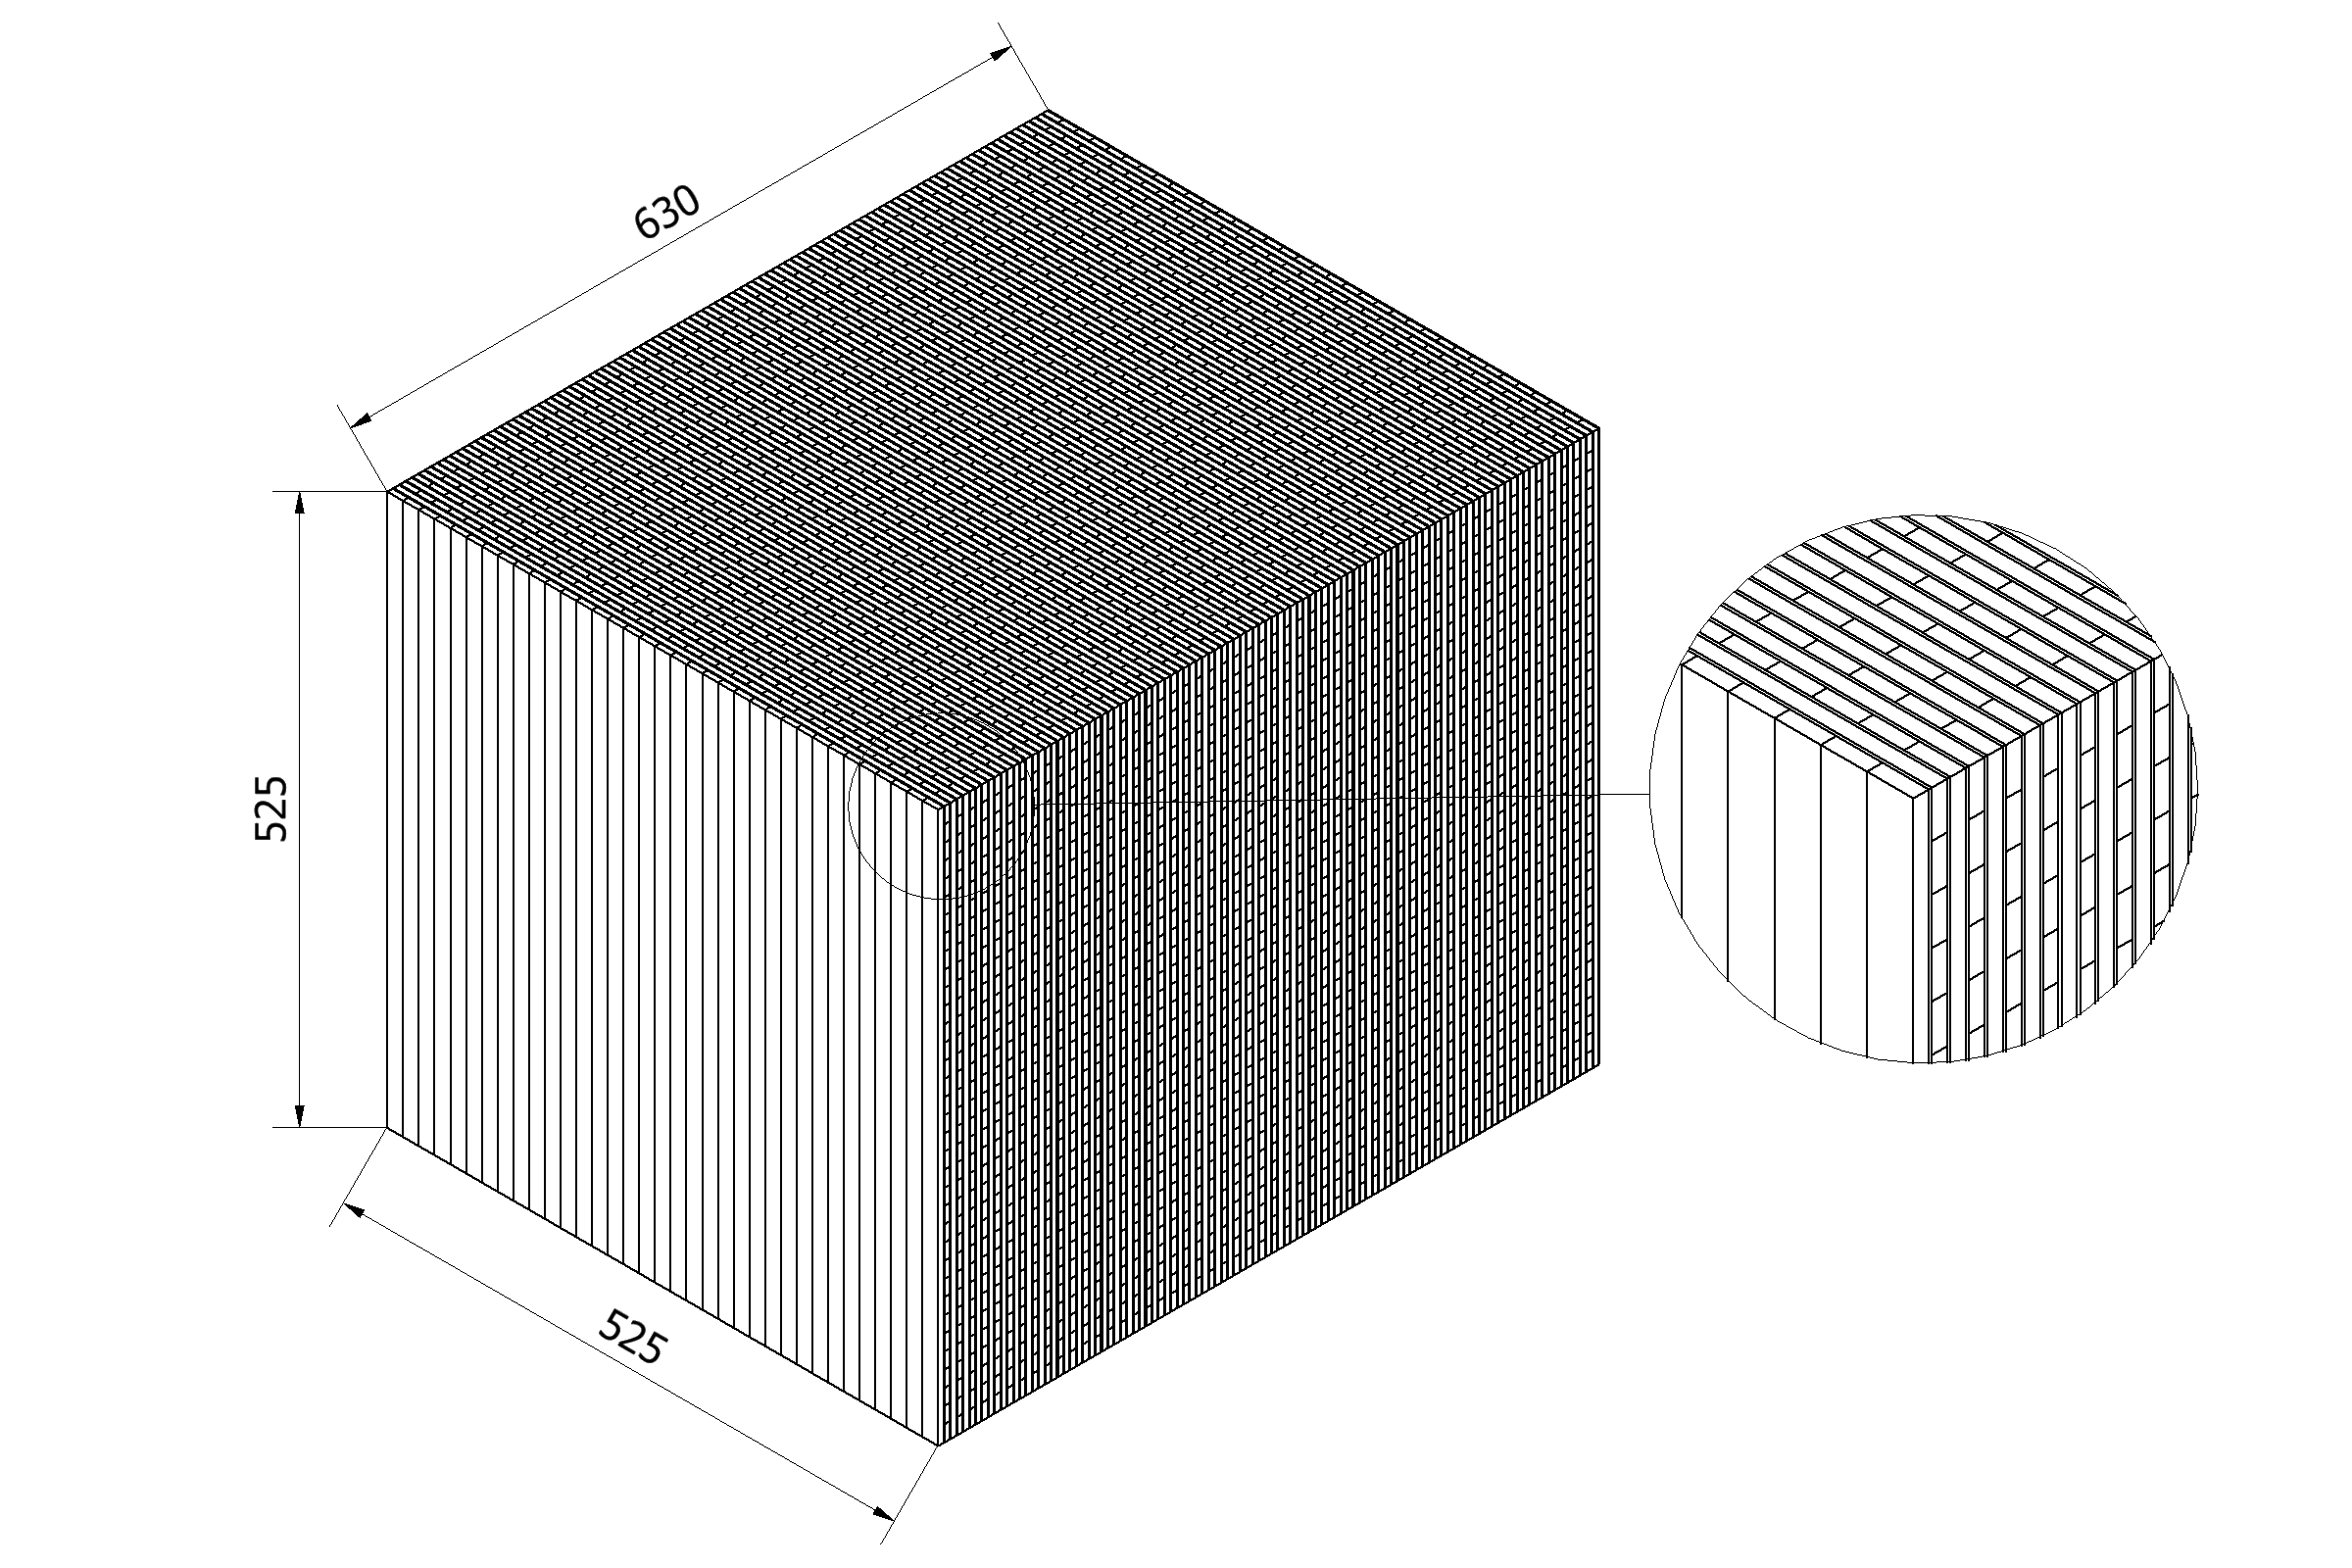
\includegraphics[width=0.6\textwidth]{figures/FullLayer_2.jpeg}
%DIFDELCMD < %%%
\DIFdelendFL \DIFaddbeginFL 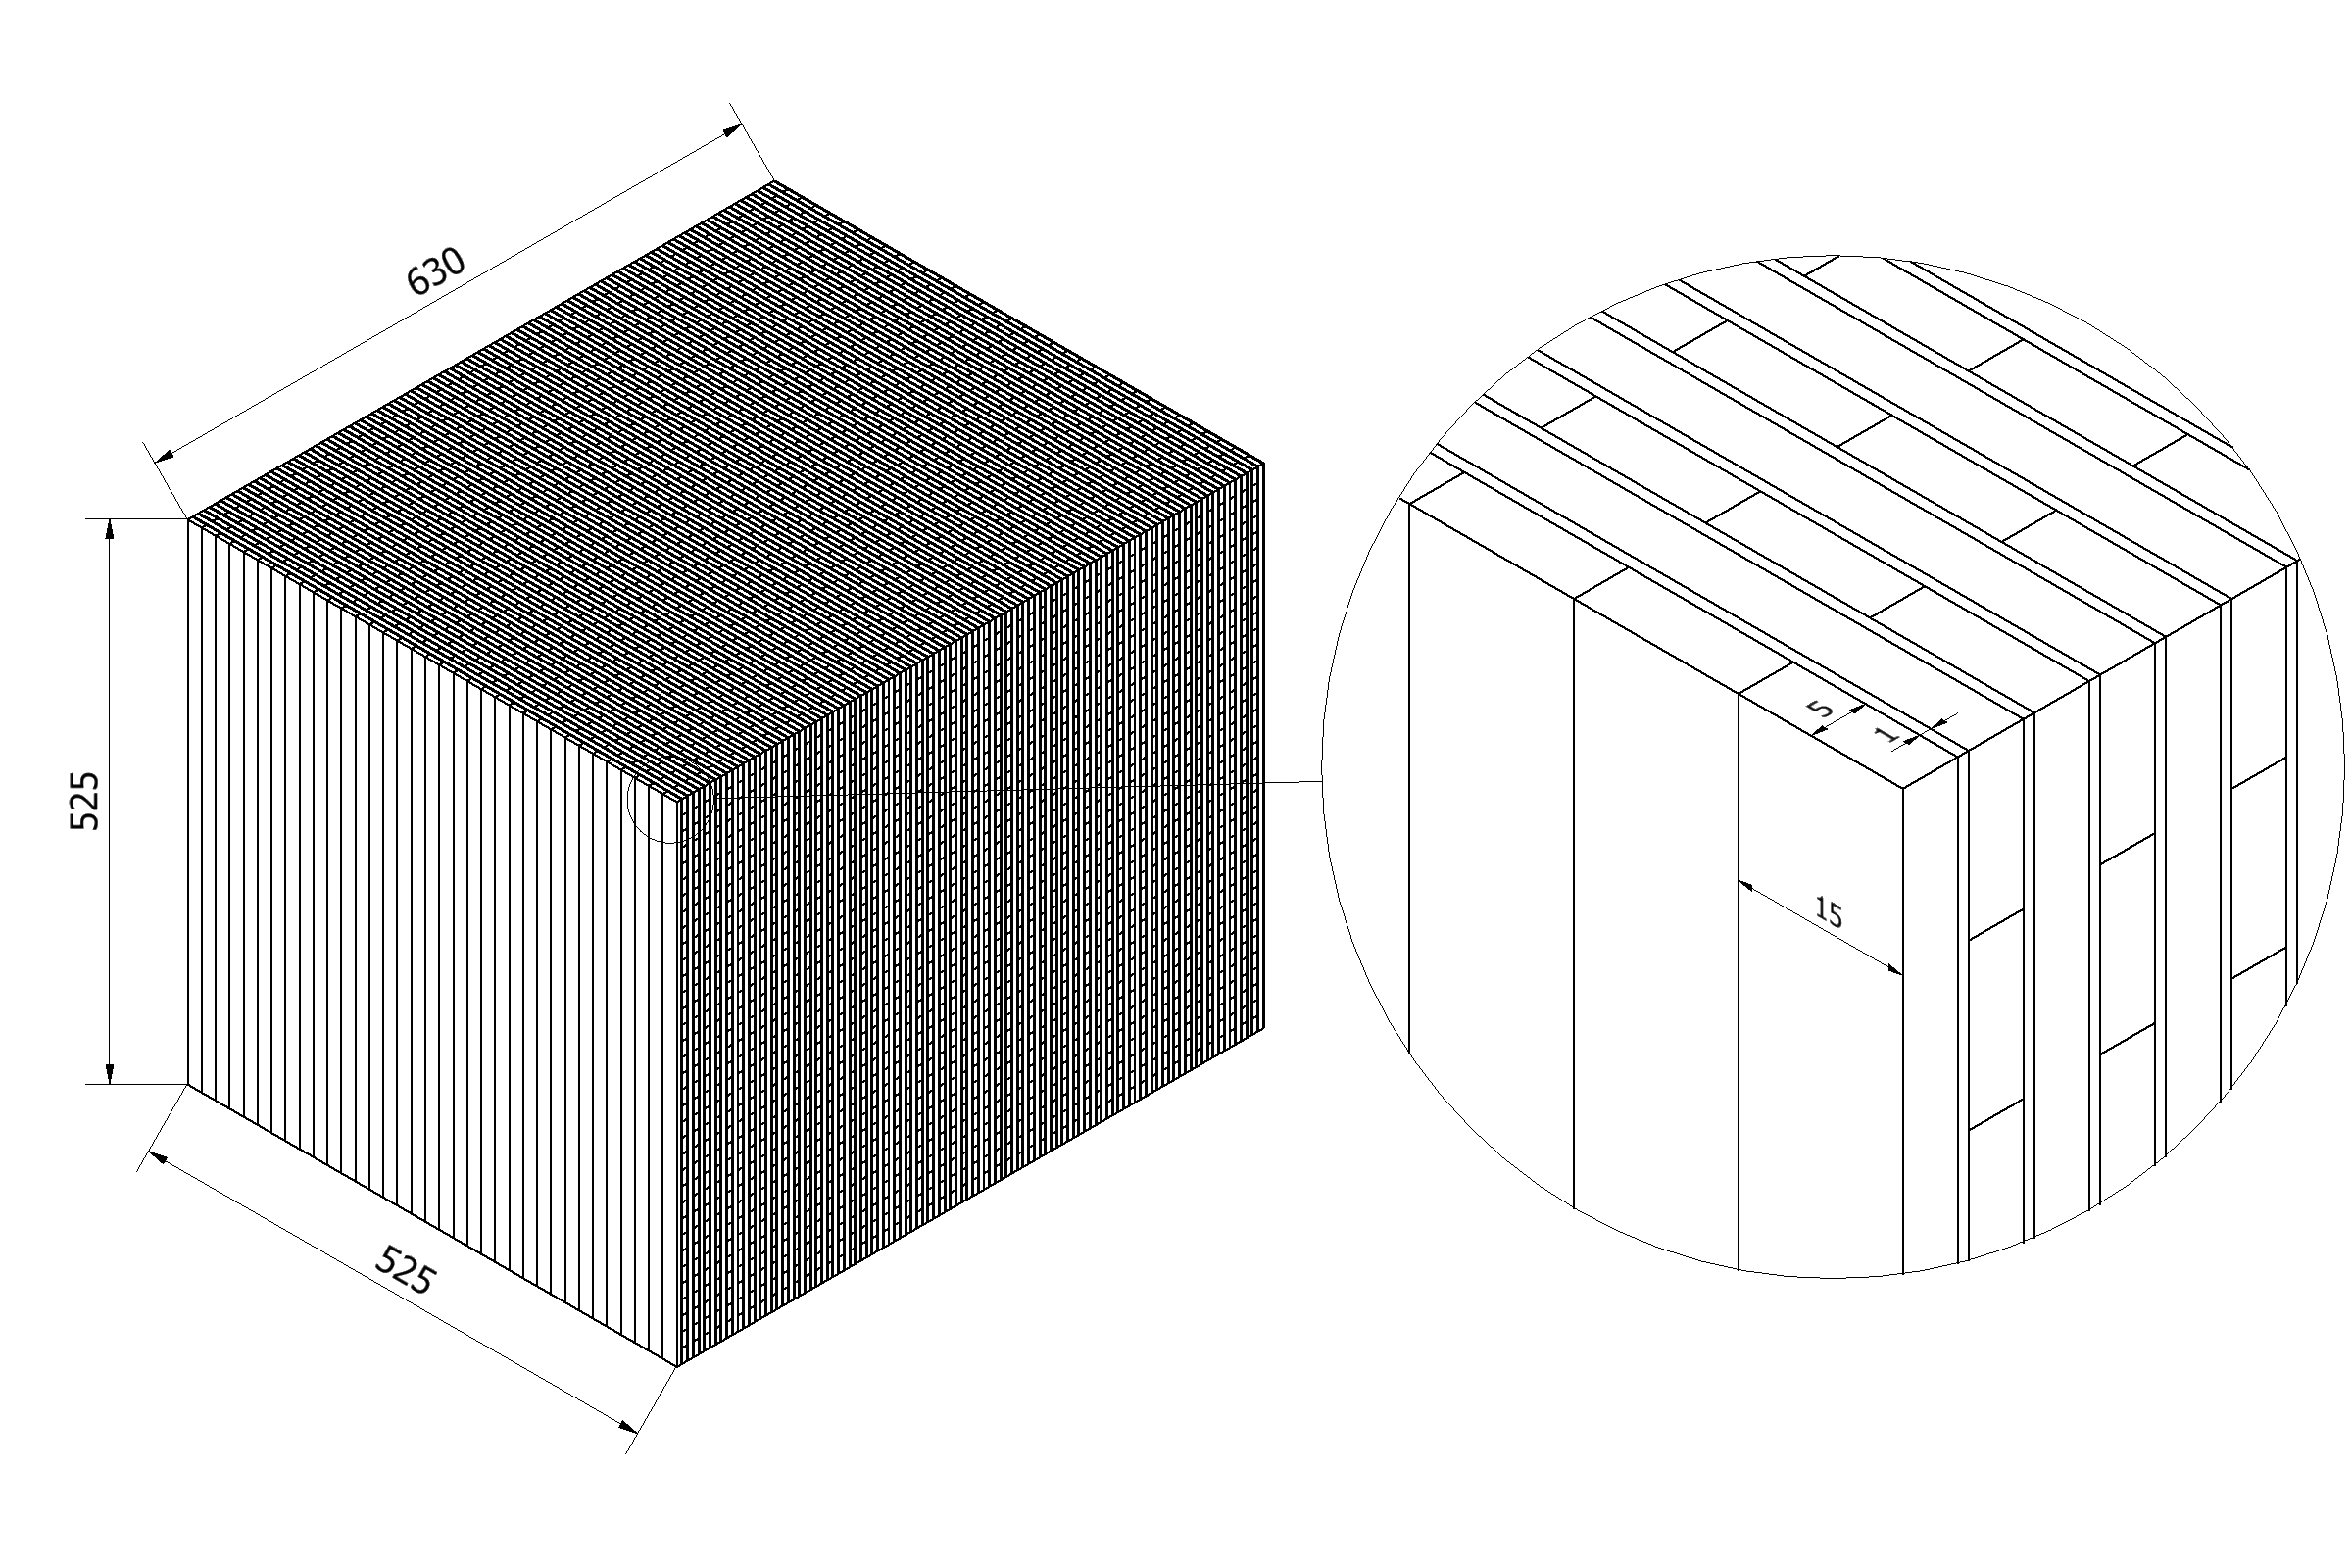
\includegraphics[width=0.6\textwidth]{figures/FullLayer_3.jpeg}
\DIFaddendFL \caption{ Schematic \DIFdelbeginFL \DIFdelFL{view }\DIFdelendFL of the sampling calorimeter \DIFdelbeginFL \DIFdelFL{. It consists }\DIFdelendFL \DIFaddbeginFL \DIFaddFL{model consisting }\DIFaddendFL of 105 alternating \DIFdelbeginFL \DIFdelFL{lead plates }\DIFdelendFL \DIFaddbeginFL \DIFaddFL{layers of a Pb plate }\DIFaddendFL and \DIFaddbeginFL \DIFaddFL{a segmented }\DIFaddendFL scintillator \DIFaddbeginFL \DIFaddFL{plate in 35 }\DIFaddendFL strips. Each scintillator \DIFdelbeginFL \DIFdelFL{layer consists of 35 scintillator strips. The cross section of each 1-mm-thick lead }\DIFdelendFL plate is \DIFdelbeginFL \DIFdelFL{525 mm $\times$ 525 mm}\DIFdelendFL \DIFaddbeginFL \DIFaddFL{oriented alternatively in horizontal and vertical directions}\DIFaddendFL . \DIFdelbeginFL \DIFdelFL{The cross section of each 5-mm-tihck scintillator strip is 525 mm $\times$ 15 mm}\DIFdelendFL \DIFaddbeginFL \DIFaddFL{See text for details}\DIFaddendFL . }
\label{fig:det_conf}
\end{figure}

\DIFdelbegin \DIFdel{The sampling calorimeter was designed as alternating }\DIFdelend \DIFaddbegin \DIFadd{Simulation models of a sampling calorimeter were constructed as a block consisting of alternating layers of a }\DIFaddend 1-mm-thick \DIFdelbegin \DIFdel{lead plates for passive converters and }\DIFdelend \DIFaddbegin \DIFadd{Pb absorber and a }\DIFaddend 5-mm-thick \DIFdelbegin \DIFdel{strips of the plastic scintillatorfor active counters. Strips are alternatively aligned along $x$ and $y$ direction }\DIFdelend \DIFaddbegin \DIFadd{polyvinyltoluene-based plastic scintillator. The plastic scintillator is segmented in 15-mm-wide strips, which is alternatively oriented in vertical and horizontal directions }\DIFaddend as shown in Fig.~\ref{fig:det_conf}. The \DIFdelbegin \DIFdel{cross section of the lead plate and the scintillator is }\DIFdelend \DIFaddbegin \DIFadd{sampling calorimeter model has a cross-section of }\DIFaddend 525\DIFdelbegin \DIFdel{mm }\DIFdelend \DIFaddbegin \DIFadd{~}\DIFaddend $\times$\DIFaddbegin \DIFadd{~}\DIFaddend 525\DIFdelbegin \DIFdel{mm and 15 mm $\times$ 525 mm, respectively. The material for the scintillator strip is polyvinyltoluene. The total number of alternating layers is 105, which corresponds to }\DIFdelend \DIFaddbegin \DIFadd{~mm$^{2}$ and accommodates 105 alternating layers of 630~mm length (}\DIFaddend 20$X_{0}$\DIFdelbegin \DIFdel{to make it possible to absorb whole products from the EM shower ranging from }\DIFdelend \DIFaddbegin \DIFadd{), which is sufficiently long to absorb full photon energy in the range of }\DIFaddend 100\DIFdelbegin \DIFdel{MeV to few GeVenergy}\DIFdelend \DIFaddbegin \DIFadd{~MeV to 2~GeV}\DIFaddend . 

\begin{figure}[!hbt]
%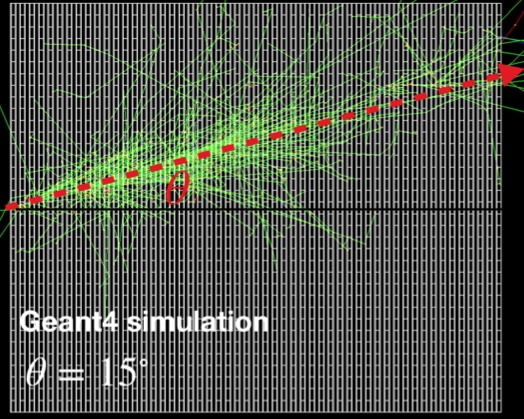
\includegraphics[width=0.45\textwidth]{figures/EventDisplay.jpg}
%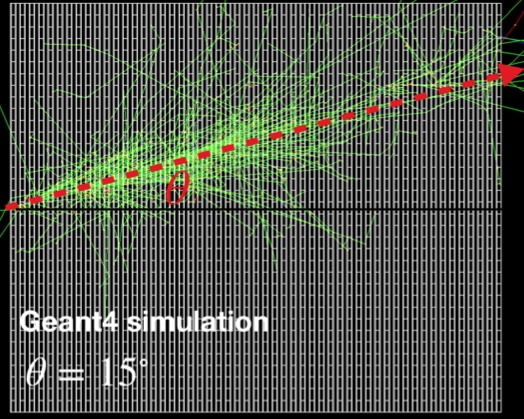
\includegraphics[width=0.45\textwidth]{figures/EventDisplay.jpg}
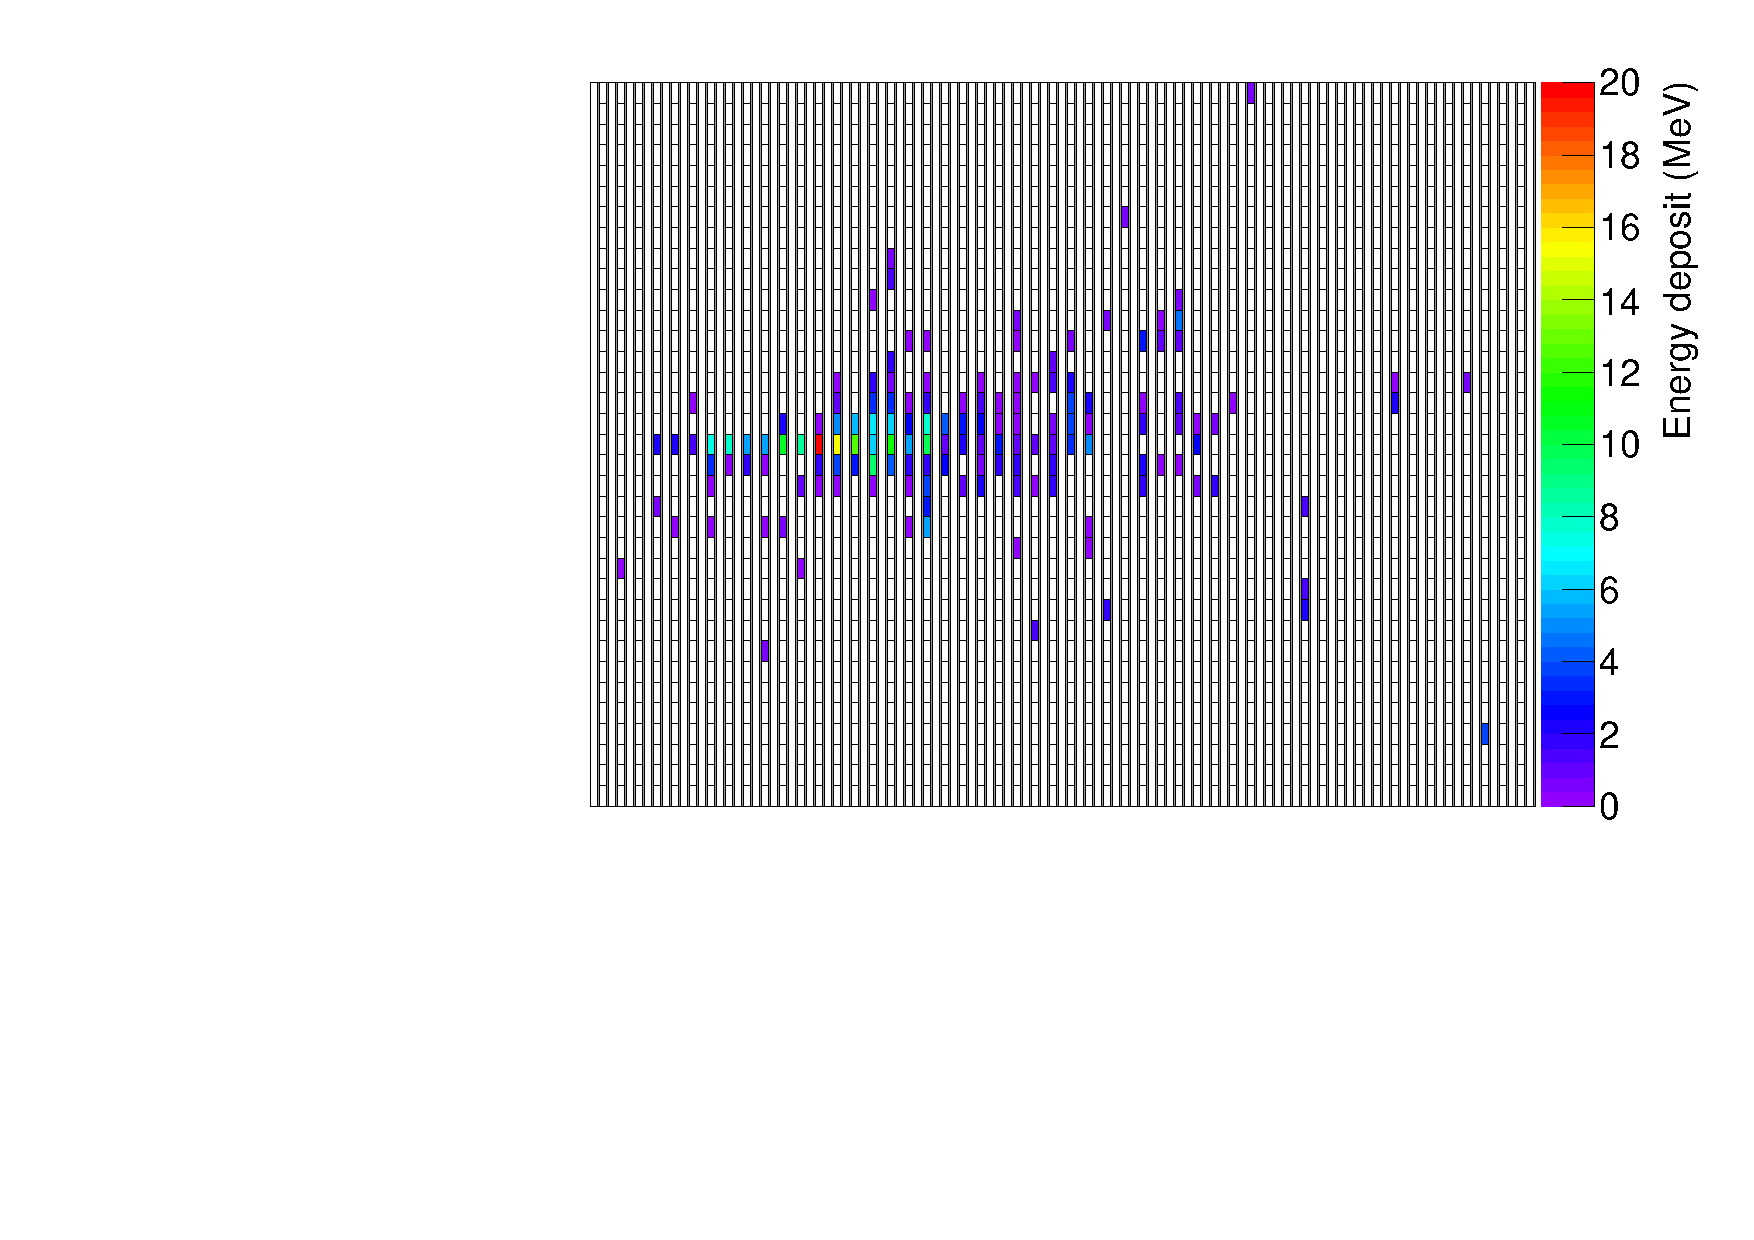
\includegraphics[width=0.48\textwidth]{figures/SingleEventXZHit.pdf}
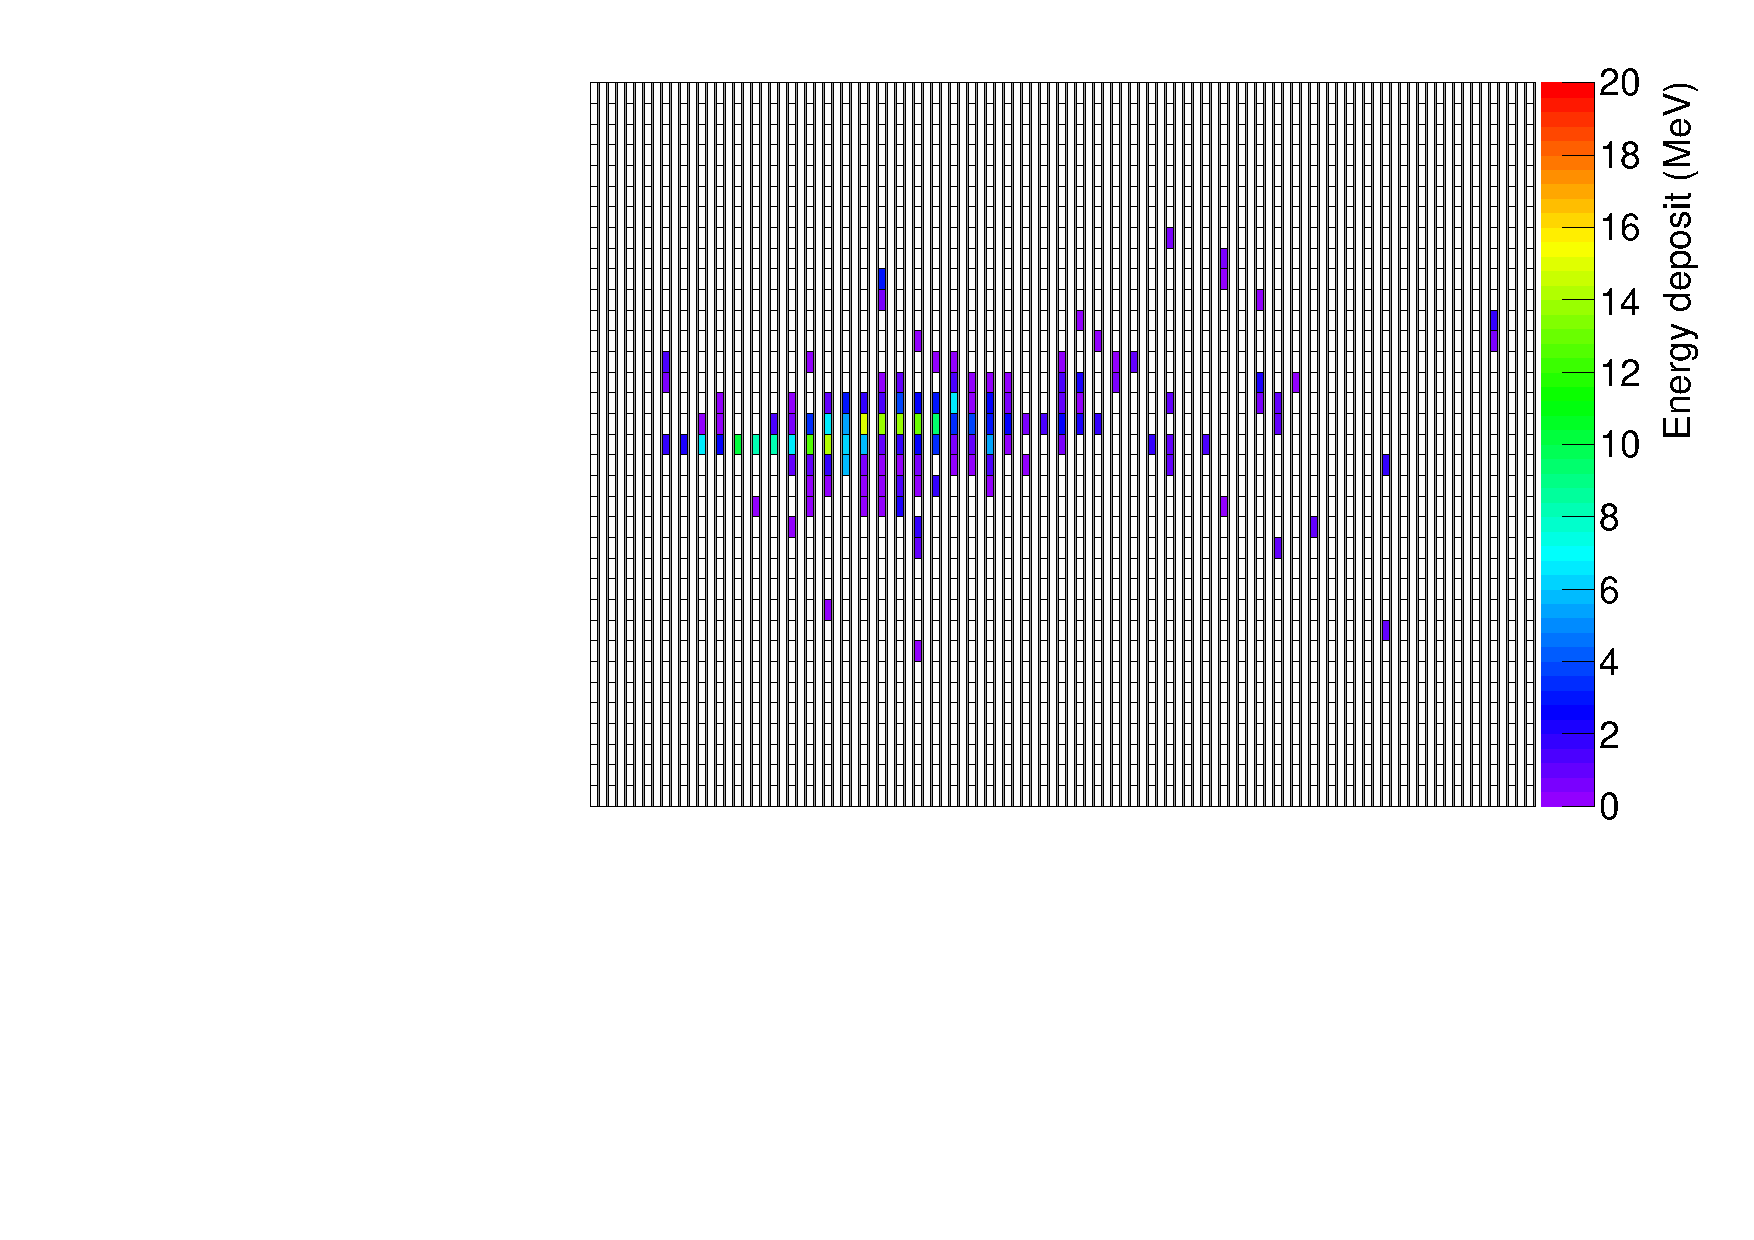
\includegraphics[width=0.48\textwidth]{figures/SingleEventYZHit.pdf}
\caption{ \DIFdelbeginFL \DIFdelFL{An event }\DIFdelendFL \DIFaddbeginFL \DIFaddFL{Event }\DIFaddendFL display of \DIFdelbeginFL \DIFdelFL{the }\DIFdelendFL \DIFaddbeginFL \DIFaddFL{simulated }\DIFaddendFL energy deposit \DIFdelbeginFL \DIFdelFL{to each scintillator strip in the $x$--$z$ plane (left) and the $y$--$z$ plane (right) }\DIFdelendFL \DIFaddbeginFL \DIFaddFL{patterns }\DIFaddendFL for \DIFdelbeginFL \DIFdelFL{the 1~GeV $\gamma$ perpendicularly }\DIFdelendFL \DIFaddbeginFL \DIFaddFL{a 1-GeV photon }\DIFaddendFL entering \DIFdelbeginFL \DIFdelFL{to }\DIFdelendFL the \DIFdelbeginFL \DIFdelFL{detector }\DIFdelendFL \DIFaddbeginFL \DIFaddFL{calorimeter }\DIFaddendFL ($\theta=$~0) \DIFaddbeginFL \DIFaddFL{in (a) $xz$- and (b) $yz$-planes}\DIFaddendFL .}
\label{fig:Evt_Dis}
\end{figure}

The \DIFdelbegin \DIFdel{interaction of incident $\gamma$ with the detector }\DIFdelend \DIFaddbegin \DIFadd{detector response to incident photons }\DIFaddend was simulated using \DIFdelbegin \DIFdel{the GEANT4 }\DIFdelend \DIFaddbegin \DIFadd{Geant4 }\DIFaddend (ver. 4.10.06) with the standard EM sub-packages~\cite{GEANT4}. The \DIFdelbegin \DIFdel{surface of the detector is defined as $z=$~0, and the $\gamma$ starts to interact with the detector. the incident angle of the $\gamma$ }\DIFdelend \DIFaddbegin \DIFadd{beam direction defines the $z$-axis. The photon direction }\DIFaddend is defined as \DIFdelbegin \DIFdel{the }\DIFdelend polar angle ($\theta$) \DIFdelbegin \DIFdel{along }\DIFdelend \DIFaddbegin \DIFadd{with respect to }\DIFaddend the $z$\DIFdelbegin \DIFdel{direction, where $\theta = 0$ case denotes that the $\gamma$ perpendicularly enters into the detector surface}\DIFdelend \DIFaddbegin \DIFadd{-axis}\DIFaddend . Figure~\ref{fig:Evt_Dis} \DIFdelbegin \DIFdel{shows the event display illustrating the energy deposit on the each scintillator strip in both of $x$--$z$ and $y$--$z$ planes for the 1~GeV~$\gamma$ with $\theta = 0$}\DIFdelend \DIFaddbegin \DIFadd{illustrates simulated energy deposit patterns in each strip for a 1-GeV photon at a normal incidence in $xz$- and $yz$-planes. Each segmented region in Fig.~\ref{fig:Evt_Dis} represents each channel}\DIFaddend .

%DIF < \begin{figure}[!hbt]
%DIF < 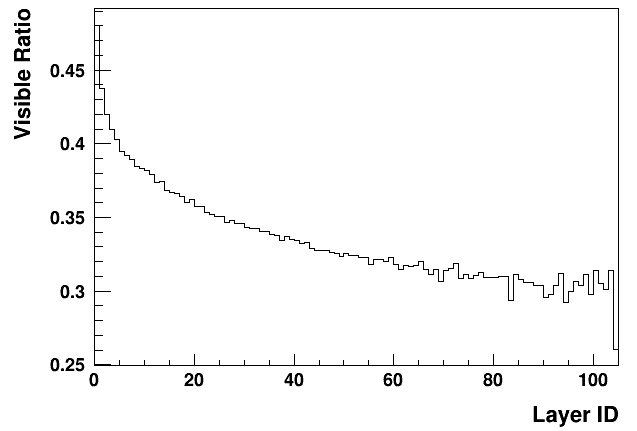
\includegraphics[width=0.48\textwidth]{figures/LayerVisibleRatio.jpg}
%DIF < 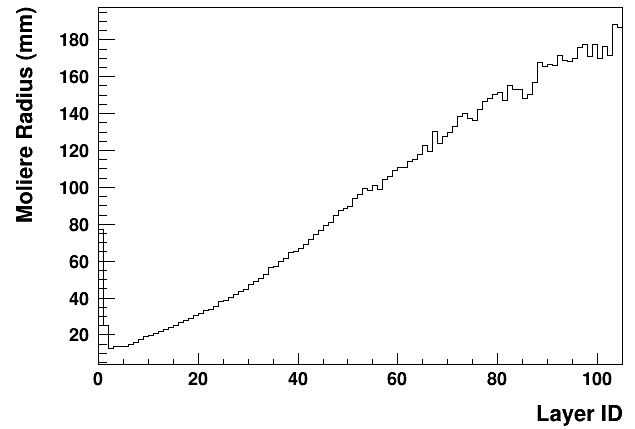
\includegraphics[width=0.48\textwidth]{figures/Moliere_layer.jpg}
%DIF < \caption{  \textcolor{red}{plots should be updated} Sampling fraction (left) and Moliere radius (right) from 1 GeV %$\gamma$ events ($\theta=0$) for each layer}
%DIF < \label{fig:sc_prop}
%DIF < \end{figure}
\DIFdelbegin %DIFDELCMD < 

%DIFDELCMD < %%%
%DIF < Figure~\ref{fig:sc_prop} shows the sampling fraction and the Moliere radius~\cite{PDG} for each layer with 1~GeV $\gamma$. In this paper, Moliere radius is defined as the distance including 90\% of (deposited) energy from the center of energy. The visible ratio (Moliere radius) decreases (increases) with increasing layer ID. It is, therefore, estimated to have better energy resolution and position separation with front layers. Note that the very front few layers are largely affected by secondaries going backward. 
%DIFDELCMD < 

%DIFDELCMD < %%%
\DIFdelend \section{\DIFdelbegin \DIFdel{ANGLE RECONSTRUCTION}\DIFdelend \DIFaddbegin \DIFadd{Reconstruction of Incidence Angles}\DIFaddend }
\label{sec:res}

\DIFdelbegin \DIFdel{The incident angle of the $\gamma$ is reconstructed with the $\XGB$, which is one of the popular machine learning toolkit providing a scalable tree boosting system}\DIFdelend \DIFaddbegin \DIFadd{Incidence angles of photons are reconstructed using the XGB model that is a scalable machine learning system for tree boosting}\DIFaddend ~\cite{xgboost:2016}. \DIFdelbegin \DIFdel{The machine learning is required to be trained. The feature, characteristic of a phenomenon, and the target, output to be predicted, are essential inputs for the training. The machine learning correlates each feature with the corresponding target for different features. Trained machine learning takes measured features and gives the target based on correlations which are made during the training. In this paper, the feature corresponds to energy deposits on }\DIFdelend \DIFaddbegin \DIFadd{A machine learning model maps a set of data inputs, known as features, to target variables. In this study, the XGB model maps a dataset of energy deposits in }\DIFaddend each scintillator strip \DIFdelbegin \DIFdel{and the target corresponds to the incident angle of the $\gamma$. }%DIFDELCMD < 

%DIFDELCMD < %%%
\DIFdel{If the feature for the training is biased, the prediction of the $\XGB$ would be correspondingly biased as the $\XGB$ reliably believes there are no biases in all features given by a user}\DIFdelend \DIFaddbegin \DIFadd{to an incidence angle of a photon. Training data were carefully prepared using Geant4 simulation such that the input datasets are representative of a detector response of real sampling calorimeters}\DIFaddend . To minimize 
\DIFdelbegin \DIFdel{this, the incident angle is uniformly generated in the range }\DIFdelend \DIFaddbegin \DIFadd{data bias, the incidence angles were uniformly generated at the detector surface in the angular range of }\DIFaddend 0\DIFdelbegin \DIFdel{to }\DIFdelend \DIFaddbegin \DIFadd{~$<\theta<$~}\DIFaddend 50\DIFdelbegin \DIFdel{degrees for incident polar angle ($\theta$) }\DIFdelend \DIFaddbegin \DIFadd{$^{\circ}$ }\DIFaddend and 0\DIFdelbegin \DIFdel{to }\DIFdelend \DIFaddbegin \DIFadd{~$<\varphi<$~}\DIFaddend 360\DIFdelbegin \DIFdel{degrees for incident azimuthal angle(}\DIFdelend \DIFaddbegin \DIFadd{$^{\circ}$, where }\DIFaddend $\varphi$ \DIFdelbegin \DIFdel{), which makes the $\XGB$ train all features we are interested in}\DIFdelend \DIFaddbegin \DIFadd{denotes azimuthal angle. Such a wide angular coverage provides good training datasets for the XGB}\DIFaddend . The number of \DIFdelbegin \DIFdel{samples for the training is $2\times10^5$ considering }\DIFdelend \DIFaddbegin \DIFadd{training samples is $10^{5}$ considering limited }\DIFaddend computing resources. To test the reconstruction of \DIFdelbegin \DIFdel{the incident angle, the incident angle is generated with the fixed }\DIFdelend \DIFaddbegin \DIFadd{incidence angles, we generated photons at a fixed incidence angle }\DIFaddend $\theta$. Note that the incident energy is known.

\begin{figure}[!hbt]
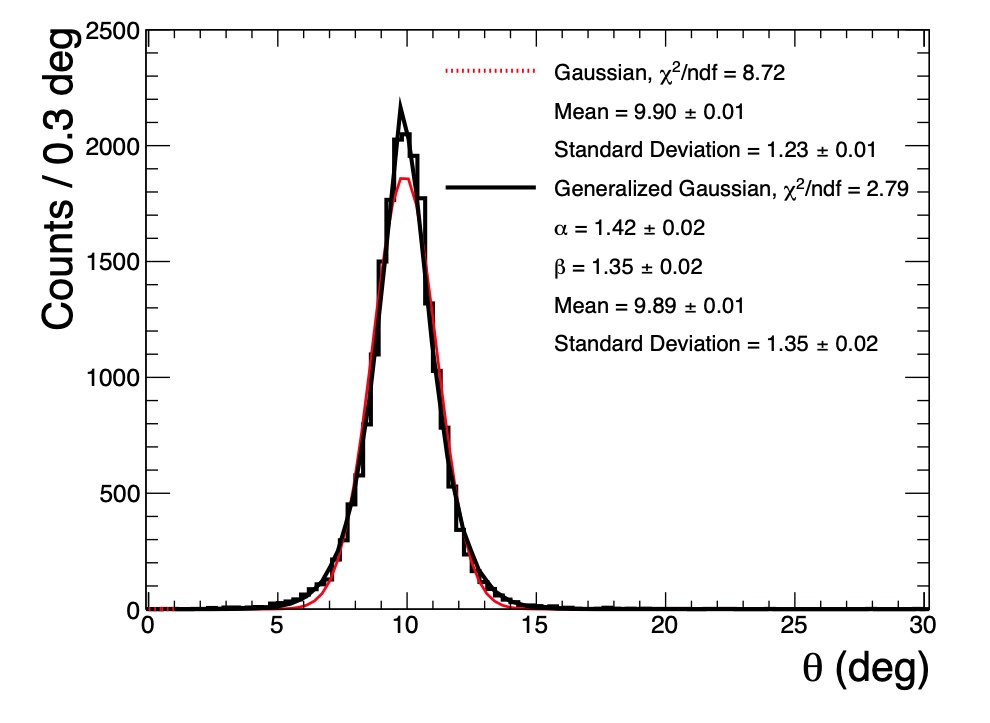
\includegraphics[width=0.7\textwidth]{figures/GG_fit.jpg}
\caption{ Reconstructed \DIFdelbeginFL \DIFdelFL{$\theta$ }\DIFdelendFL \DIFaddbeginFL \DIFaddFL{polar angle }\DIFaddendFL distribution for \DIFaddbeginFL \DIFaddFL{1-GeV photons generated at }\DIFaddendFL $\theta=$~10\DIFdelbeginFL \DIFdelFL{~deg events}\DIFdelendFL \DIFaddbeginFL \DIFaddFL{$^{\circ}$}\DIFaddendFL . The distribution is fitted with the Gaussian \DIFdelbeginFL \DIFdelFL{function }\DIFdelendFL and the Generalized Gaussian function. The \DIFdelbeginFL \DIFdelFL{Generalized Gaussian function provides }\DIFdelendFL \DIFaddbeginFL \DIFaddFL{later gives a }\DIFaddendFL better \DIFdelbeginFL \DIFdelFL{description for both tails}\DIFdelendFL \DIFaddbeginFL \DIFaddFL{result}\DIFaddendFL .}
\label{fig:angle_10degree}
\end{figure}

Figure~\ref{fig:angle_10degree} \DIFdelbegin \DIFdel{shows reconstructed }\DIFdelend \DIFaddbegin \DIFadd{represents a distribution of reconstructed incidence angles }\DIFaddend $\theta$ for \DIFdelbegin \DIFdel{1~GeV $\gamma$ with }\DIFdelend \DIFaddbegin \DIFadd{1-GeV photons generated at }\DIFaddend $\theta=$~10\DIFdelbegin \DIFdel{~degrees}\DIFdelend \DIFaddbegin \DIFadd{$^{\circ}$}\DIFaddend . The distribution is fitted with the Gaussian function and the Generalized Gaussian (GG) function. \DIFdelbegin \DIFdel{GG function provides better description for both tails of the }\DIFdelend \DIFaddbegin \DIFadd{We tested two functions, Gaussian and GG to describe the reconstructed angle }\DIFaddend distribution. The GG function\DIFdelbegin \DIFdel{can be expressed as
}\begin{displaymath} 
\DIFdel{f(x; \mu, \alpha, \beta) = \frac{\beta}{2 \alpha \Gamma(1/\beta)}e^{-(|x-\mu|/\alpha)^\beta}
}\end{displaymath}%DIFAUXCMD
\DIFdelend \DIFaddbegin \DIFadd{, also known as the generalized error distribution, is expressed as
}\begin{eqnarray} 
\DIFadd{f(x; \mu, \alpha, \beta) = \frac{\beta}{2 \alpha \Gamma(1/\beta)}e^{-(|x-\mu|/\alpha)^\beta},
\label{eqn:gg}
}\end{eqnarray}\DIFaddend 
\DIFdelbegin \DIFdel{The variation of the GG function can be expressed as, then, }\DIFdelend \DIFaddbegin \DIFadd{where $\mu$ denotes a mean value. Parameters $\alpha$ and $\beta$ determine the scale and shape of the distribution, respectively. Variance of the GG function is given by }\DIFaddend $\sigma^2 \equiv \alpha^2 \Gamma(3/\beta) / \Gamma(1/\beta)$. The angular resolution of the \DIFdelbegin \DIFdel{incident }\DIFdelend \DIFaddbegin \DIFadd{incidence }\DIFaddend angle reconstruction is defined as $\sigma$.

\begin{figure}[!hbt]
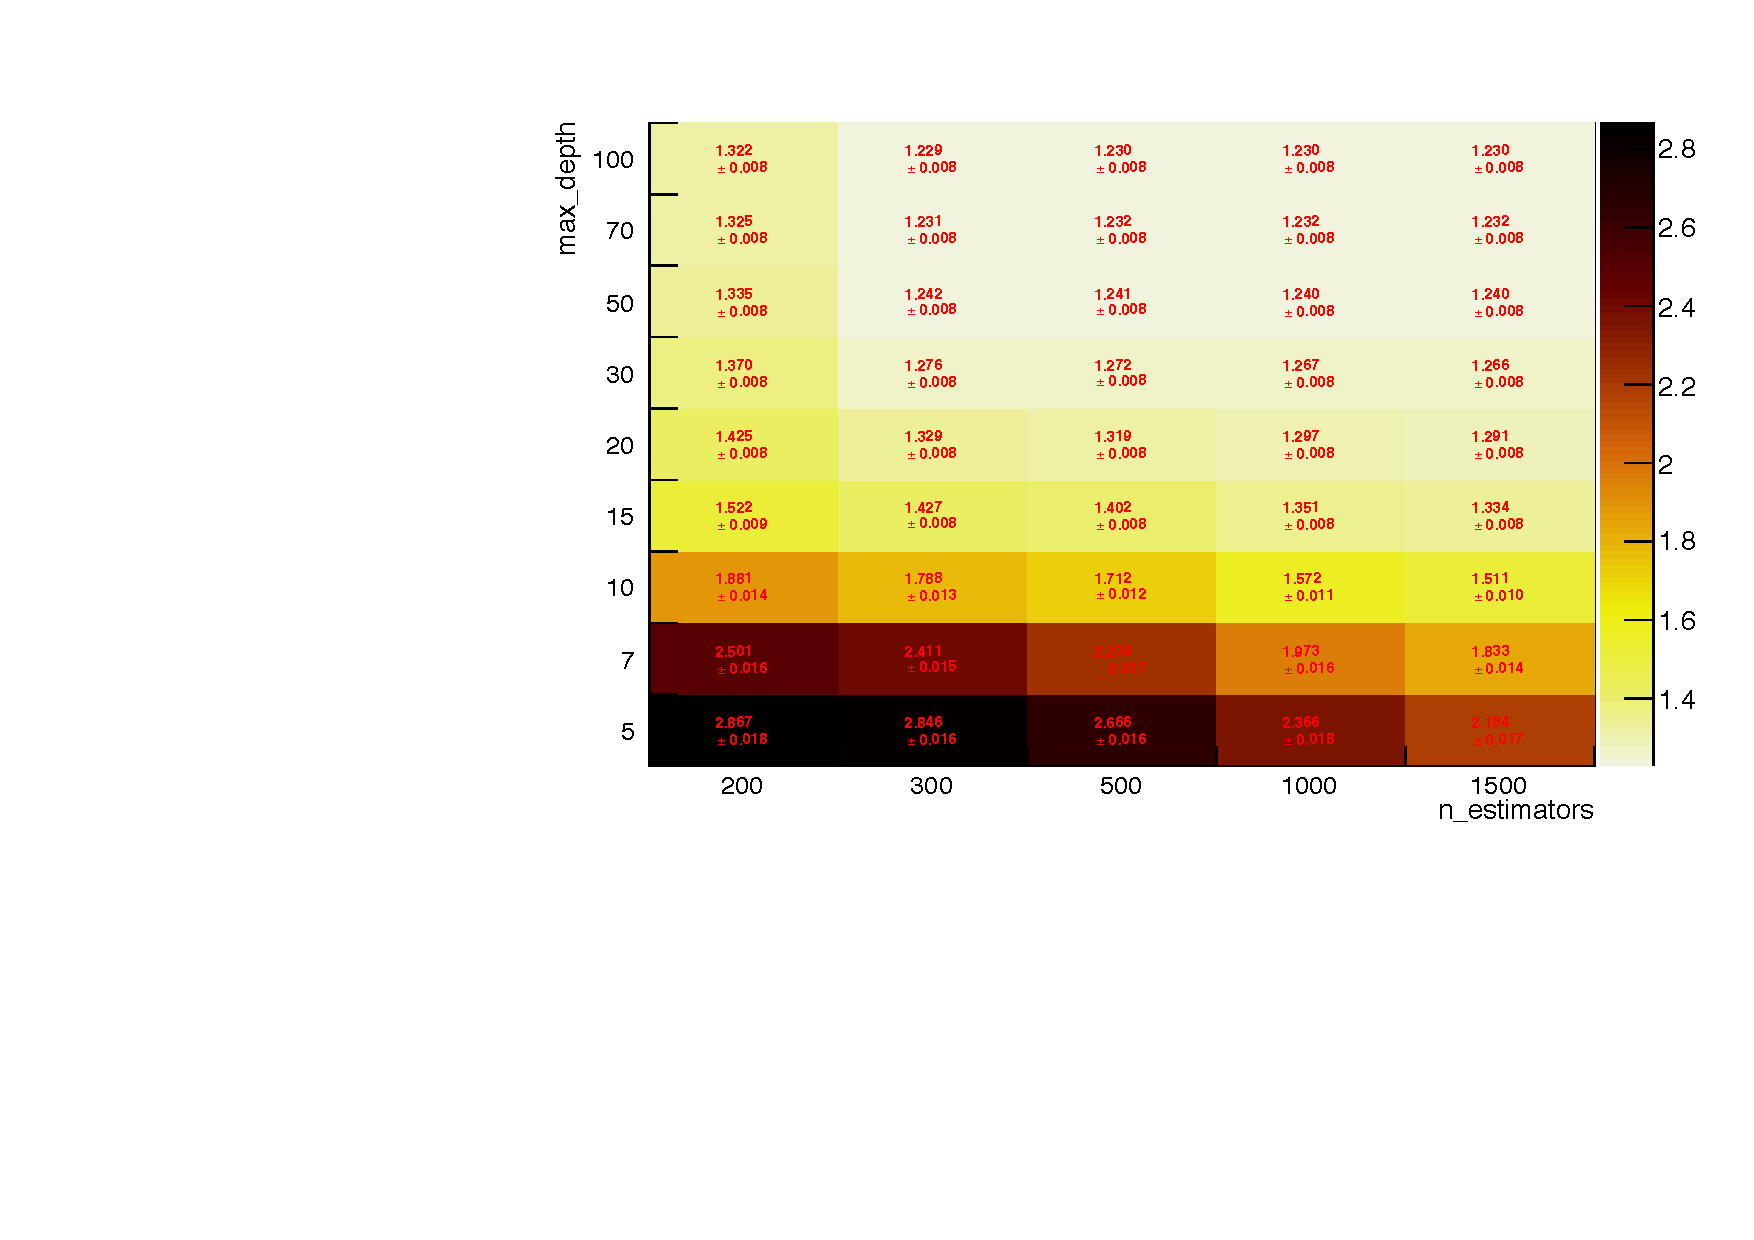
\includegraphics[width=0.89\textwidth]{figures/optimization_plot.pdf}
\caption{\DIFdelbeginFL \DIFdelFL{The angular resolution for the varying }\DIFdelendFL \DIFaddbeginFL \DIFaddFL{Angular resolutions are displayed in terms of combination of }\DIFaddendFL N\_estimators and \DIFdelbeginFL \DIFdelFL{the varying }\DIFdelendFL Max. depth. The best angular resolution is obtained with N\_estimators~=~300 and Max. depth~=~100. }
\label{fig:par_scan}
\end{figure}

\DIFdelbegin \DIFdel{As the reconstruction of the incident angle depends on hyperparameters of the $\XGB$, which controls the details of training processes, dedicated tests to optimize the hyperparameter were executed. It is assumed that a set of hyperperameters providing the best angular resolutionwould be optimized}\DIFdelend \DIFaddbegin \DIFadd{We studied a correlation between byperparameters of the XGB model and the angular resolution}\DIFaddend . The test scans the evaluated angular resolution with different hyperparameters. Figure~\ref{fig:par_scan} shows the \DIFdelbegin \DIFdel{result of the test for }\DIFdelend \DIFaddbegin \DIFadd{test results with }\DIFaddend N\_estimators and Max. depth. N\_estimators defines \DIFdelbegin \DIFdel{allowed maximal }\DIFdelend \DIFaddbegin \DIFadd{the maximum allowed }\DIFaddend number of decision trees \DIFaddbegin \DIFadd{to be developed}\DIFaddend , and the Max. depth defines \DIFaddbegin \DIFadd{the }\DIFaddend complexity of the structure of decision trees. The \DIFaddbegin \DIFadd{best hyperparameter combination was searched for in terms of the angular resolution. As a results, }\DIFaddend N\_estimators and Max. depth are \DIFdelbegin \DIFdel{determined to be }\DIFdelend \DIFaddbegin \DIFadd{set to }\DIFaddend 300 and 100, respectively. Similar tests \DIFdelbegin \DIFdel{are applied to different hyperparameters, and definitive values for each hyperparameter are shown }\DIFdelend \DIFaddbegin \DIFadd{were also performed for different hyperparameters. The best values for other hyperparameters are displayed }\DIFaddend in Tab~\ref{tab:XgbPar}. \DIFaddbegin \DIFadd{Other hyperparameters tuned in this study are Subsample, Learning rate, and Gamma. Subsample controls the fraction of total event samples for each boosting procedure, and Learning rate weights a decision tree to be added current model. Lastly, Gamma regulates the evaluation of each decision tree.
}\DIFaddend 

\begin{table}[hbt!]
\centering
\caption{Hyperparameters of the $\XGB$}
\begin{tabular}{cccc}
\hline 
Parameter & Function & Default value & Used value \\ \hline 
N\_estimators & The number of decision trees & N.A. & 300 \\  
Max. depth & Possible maximum depth of tree structure & 6 & 100 \\ 
Subsample & Fraction of total data used for a single decision & 1 & 0.8 \\ 
Learning rate & Step length for calculation & 0.3 & 0.02 \\ 
Gamma & Requirement on minimum loss function & 0 & 0 \\ 
\hline
\end{tabular}
\label{tab:XgbPar}
\end{table}

\begin{figure}[!hbt]
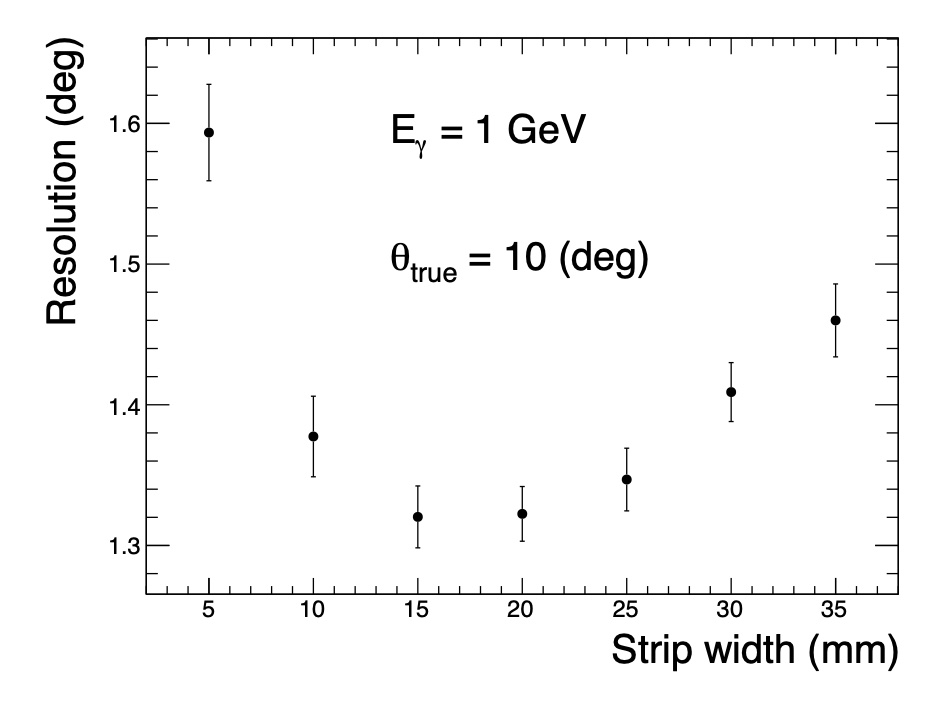
\includegraphics[width=0.58\textwidth]{figures/res_width.jpg}
\caption{ \DIFdelbeginFL \DIFdelFL{The angular resolution as a function }\DIFdelendFL \DIFaddbeginFL \DIFaddFL{Angular resolutions are deduced in terms }\DIFaddendFL of the \DIFdelbeginFL \DIFdelFL{scintillator }\DIFdelendFL strip width for \DIFdelbeginFL \DIFdelFL{1~GeV $\gamma$ with }\DIFdelendFL \DIFaddbeginFL \DIFaddFL{1-GeV photons at }\DIFaddendFL $\theta=$~10\DIFdelbeginFL \DIFdelFL{~deg. The angular resolution is optimized with 15- to 20-mm-wide strips.}\DIFdelendFL \DIFaddbeginFL \DIFaddFL{$^{\circ}$ }\DIFaddendFL }
\label{fig:angle_reco_width}
\end{figure}

\DIFdelbegin \DIFdel{The angular resolution was evaluated with the width of scintillator strips varying }\DIFdelend \DIFaddbegin \DIFadd{Angular resolutions were deduced with varying strip widths }\DIFaddend from 5 mm to 35 mm \DIFaddbegin \DIFadd{as shown in Fig.~\ref{fig:angle_reco_width}}\DIFaddend . \DIFdelbegin \DIFdel{Figure~\ref{fig:angle_reco_width}shows the angular resolution as a function of the width. }\DIFdelend \DIFaddbegin \DIFadd{The }\DIFaddend 15-mm-wide strips \DIFdelbegin \DIFdel{provide }\DIFdelend \DIFaddbegin \DIFadd{yield }\DIFaddend the best angular resolution \DIFdelbegin \DIFdel{. The width longer than 15 mm suffers from the dilution of the EM shower, resulting in worse resolution. On the other hand, the width shorter than 15 mm results in }\DIFdelend \DIFaddbegin \DIFadd{of 1.23~$\pm$~0.01$^{\circ}$. The shorter the strip width is, the }\DIFaddend larger size of features, which \DIFdelbegin \DIFdel{causes a negative influence on the }\DIFdelend \DIFaddbegin \DIFadd{can influence negatively in }\DIFaddend machine learning. \DIFdelbegin \DIFdel{Dedicated study is described in fig~\ref{fig:angle_reco_width}}\DIFdelend \DIFaddbegin \DIFadd{For longer strips, the EM shower information can hardly be obtained}\DIFaddend .

\begin{figure}[!hbt]
\DIFdelbeginFL %DIFDELCMD < 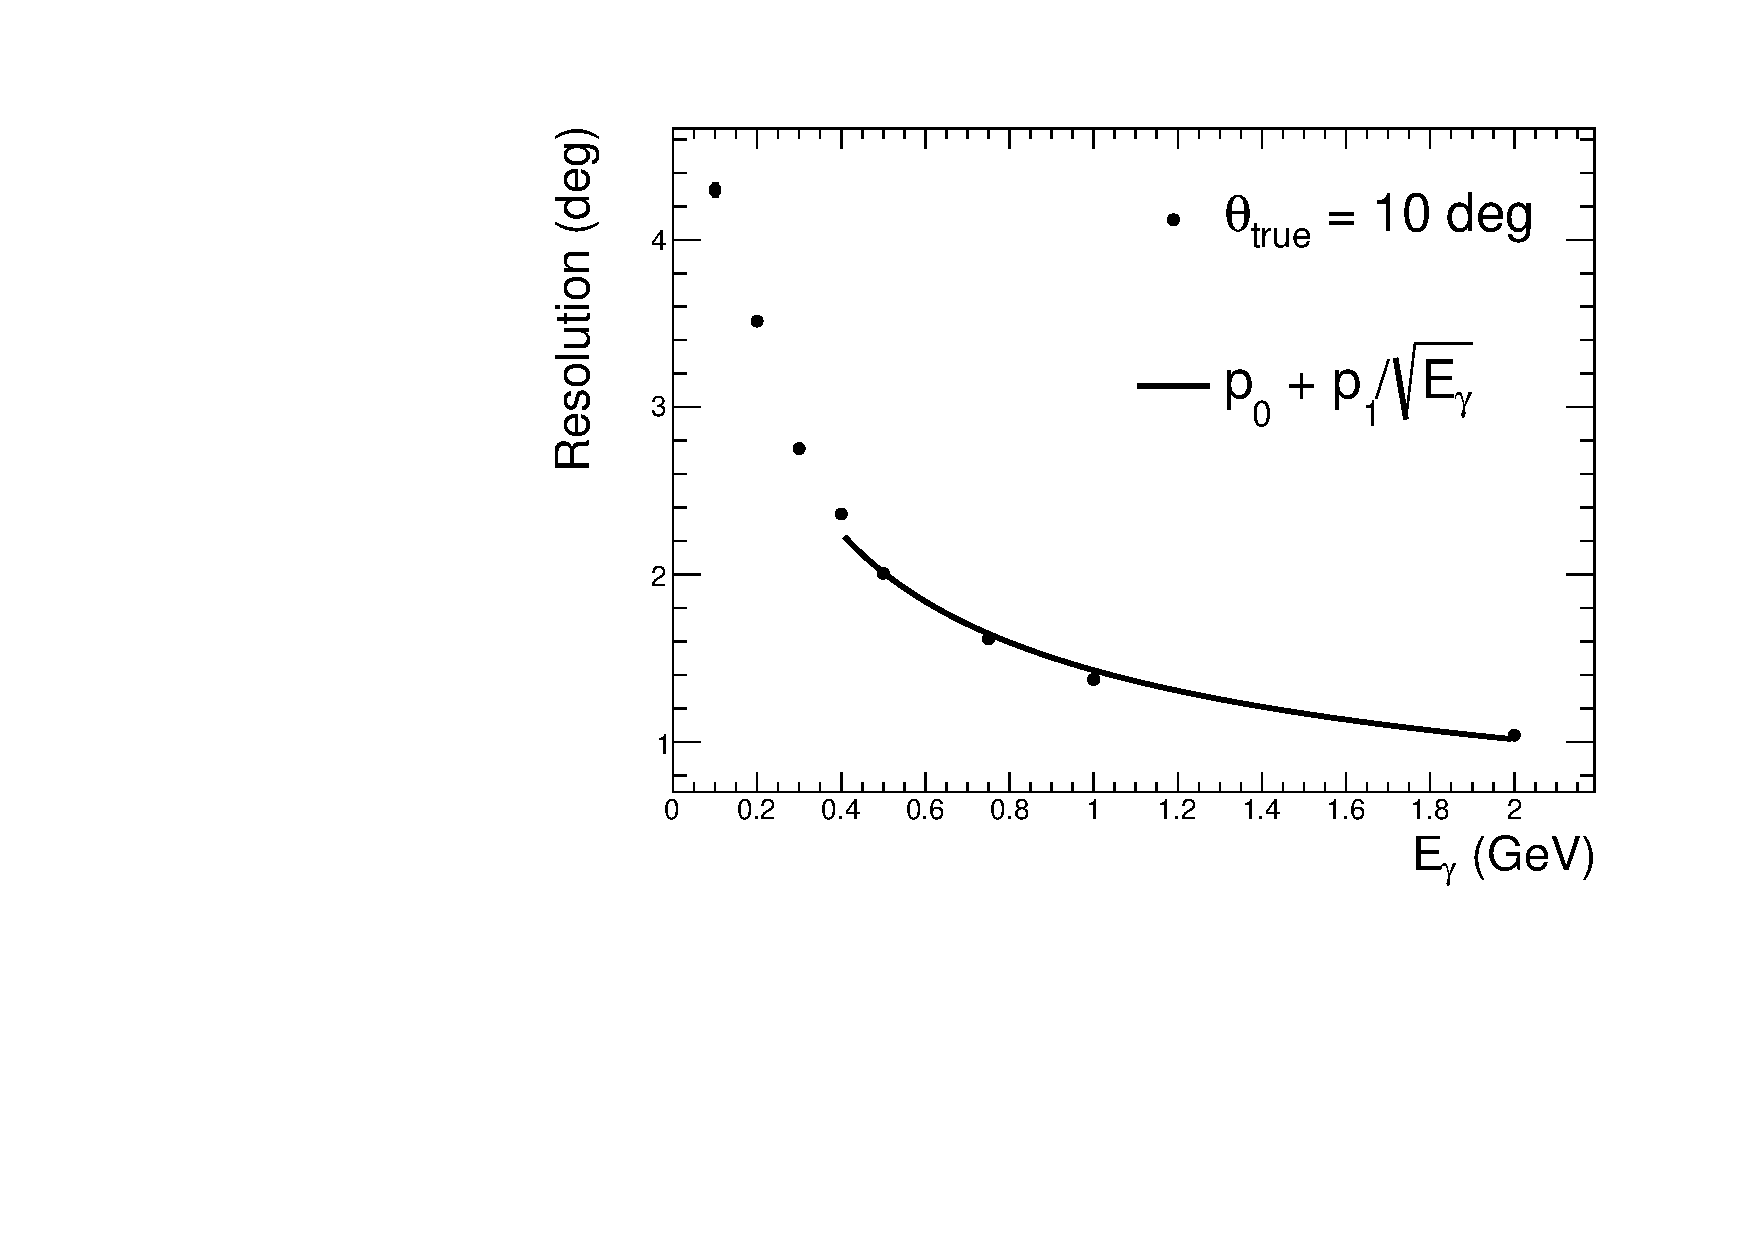
\includegraphics[width=0.48\textwidth]{figures/Fig5_reco_graph.pdf}
%DIFDELCMD < 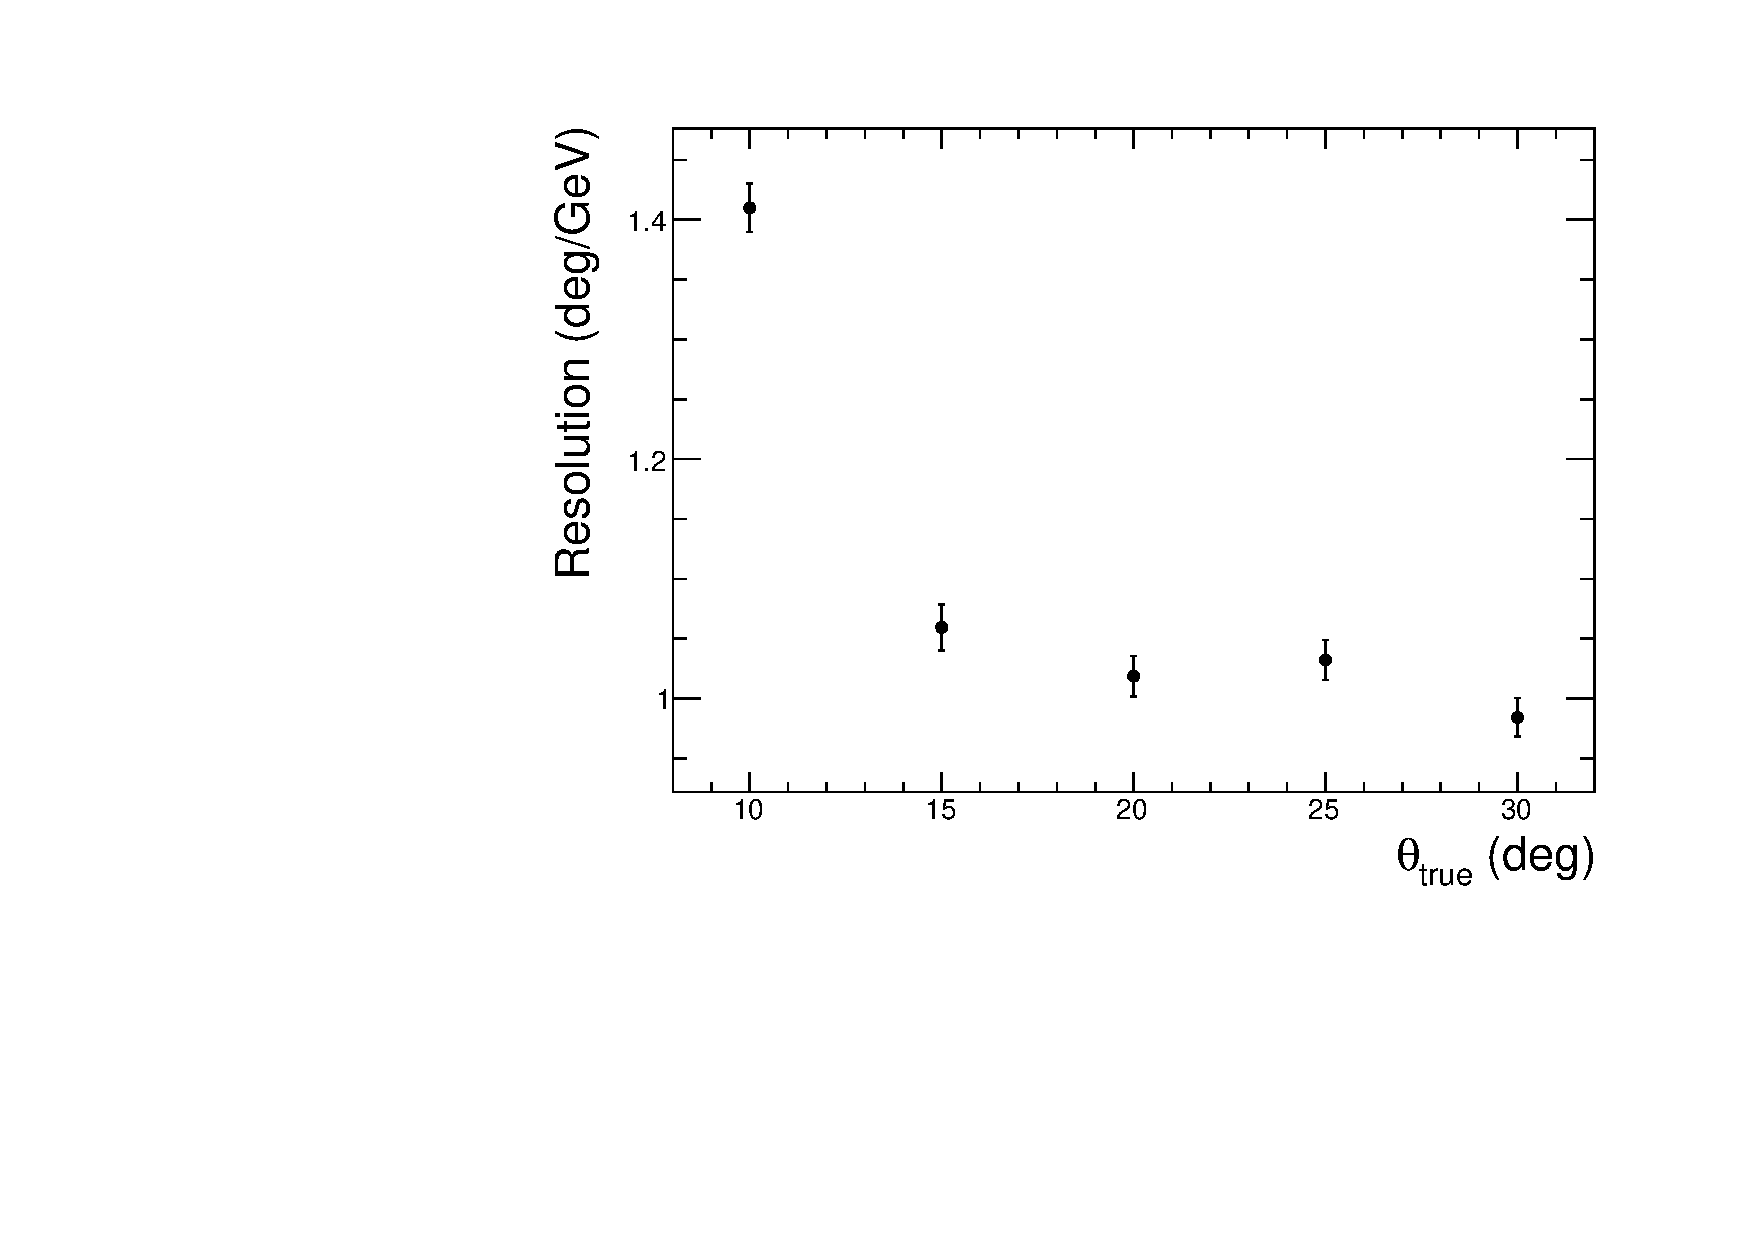
\includegraphics[width=0.48\textwidth]{figures/Fig5_reco_inc.pdf}
%DIFDELCMD < %%%
\DIFdelendFL \DIFaddbeginFL \centering
\stackinset{c}{0.cm}{b}{-0.4cm}{(a)}{
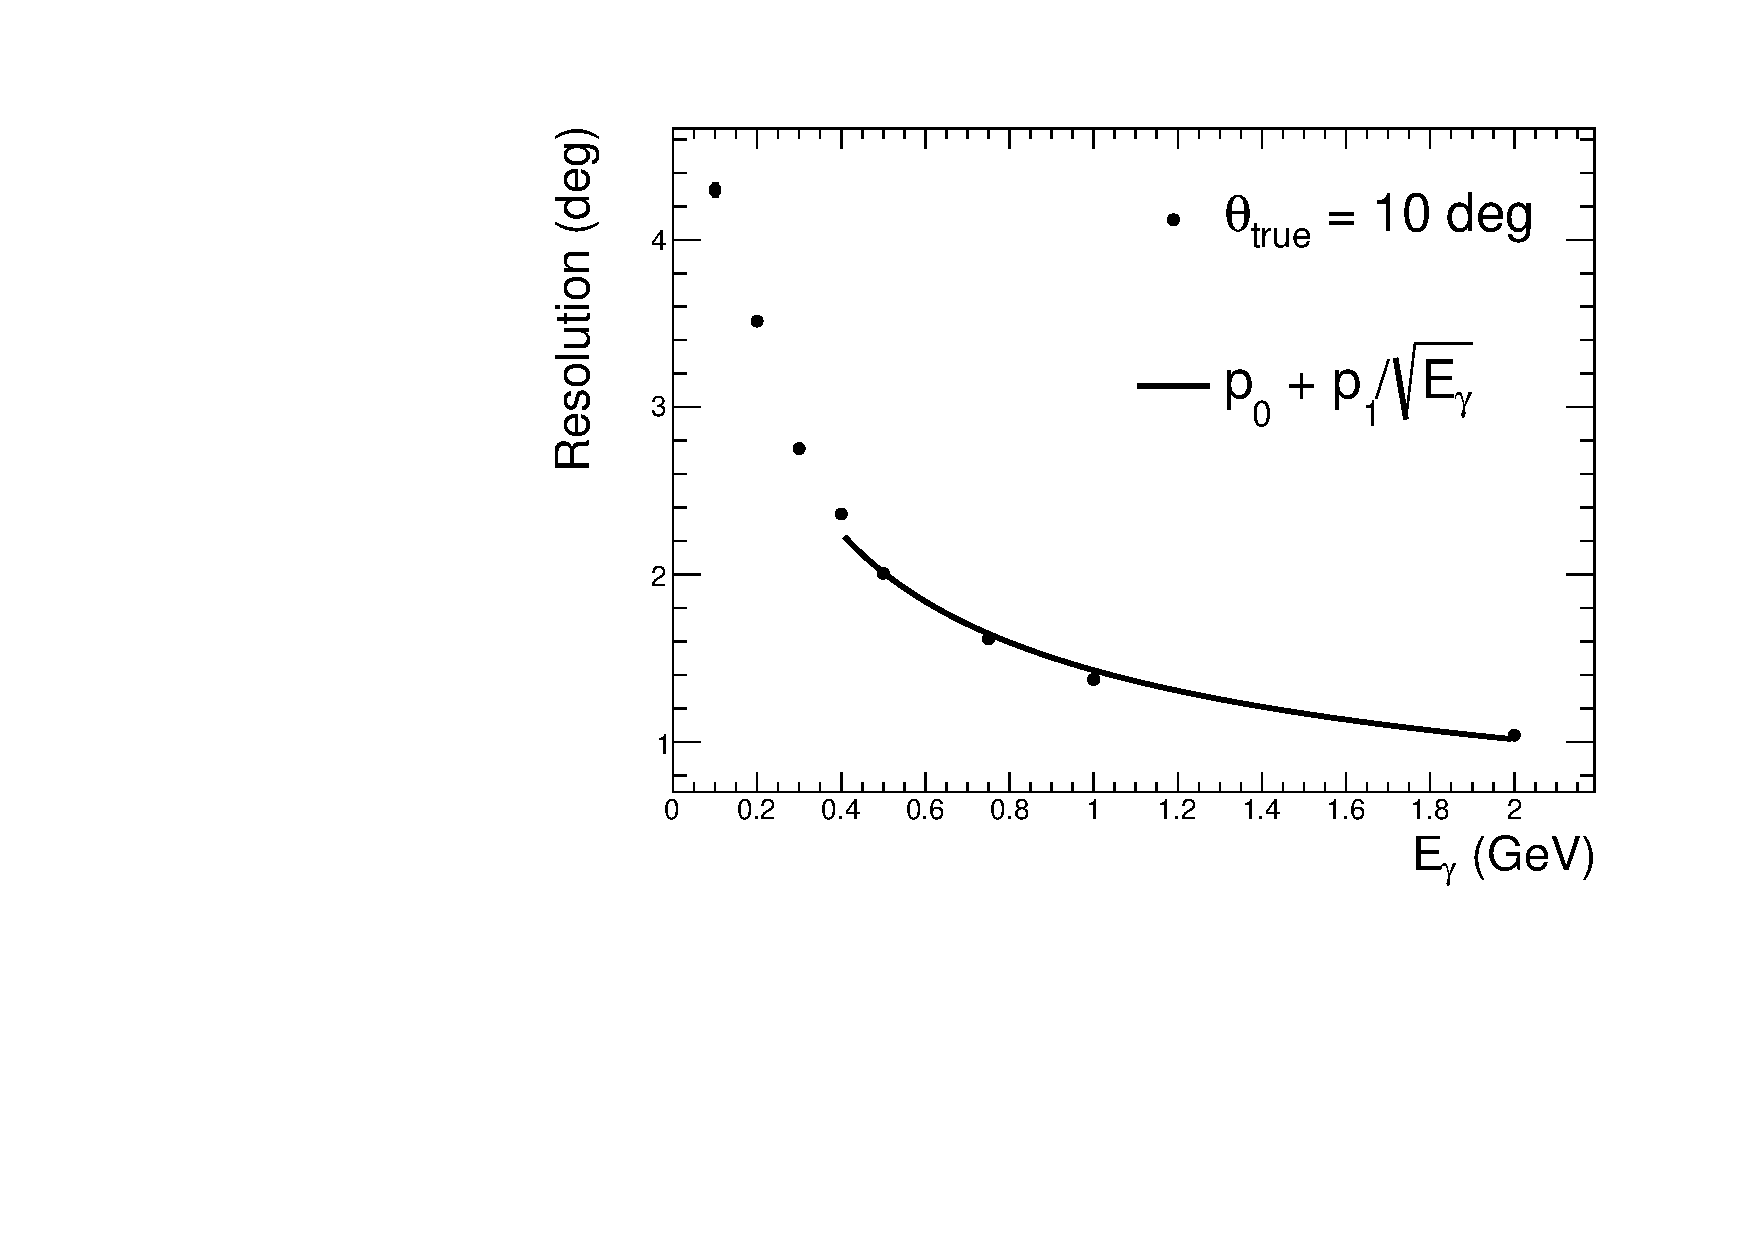
\includegraphics[width=0.48\textwidth]{figures/Fig5_reco_graph.pdf}
}\stackinset{c}{0.cm}{b}{-0.4cm}{(b)}{
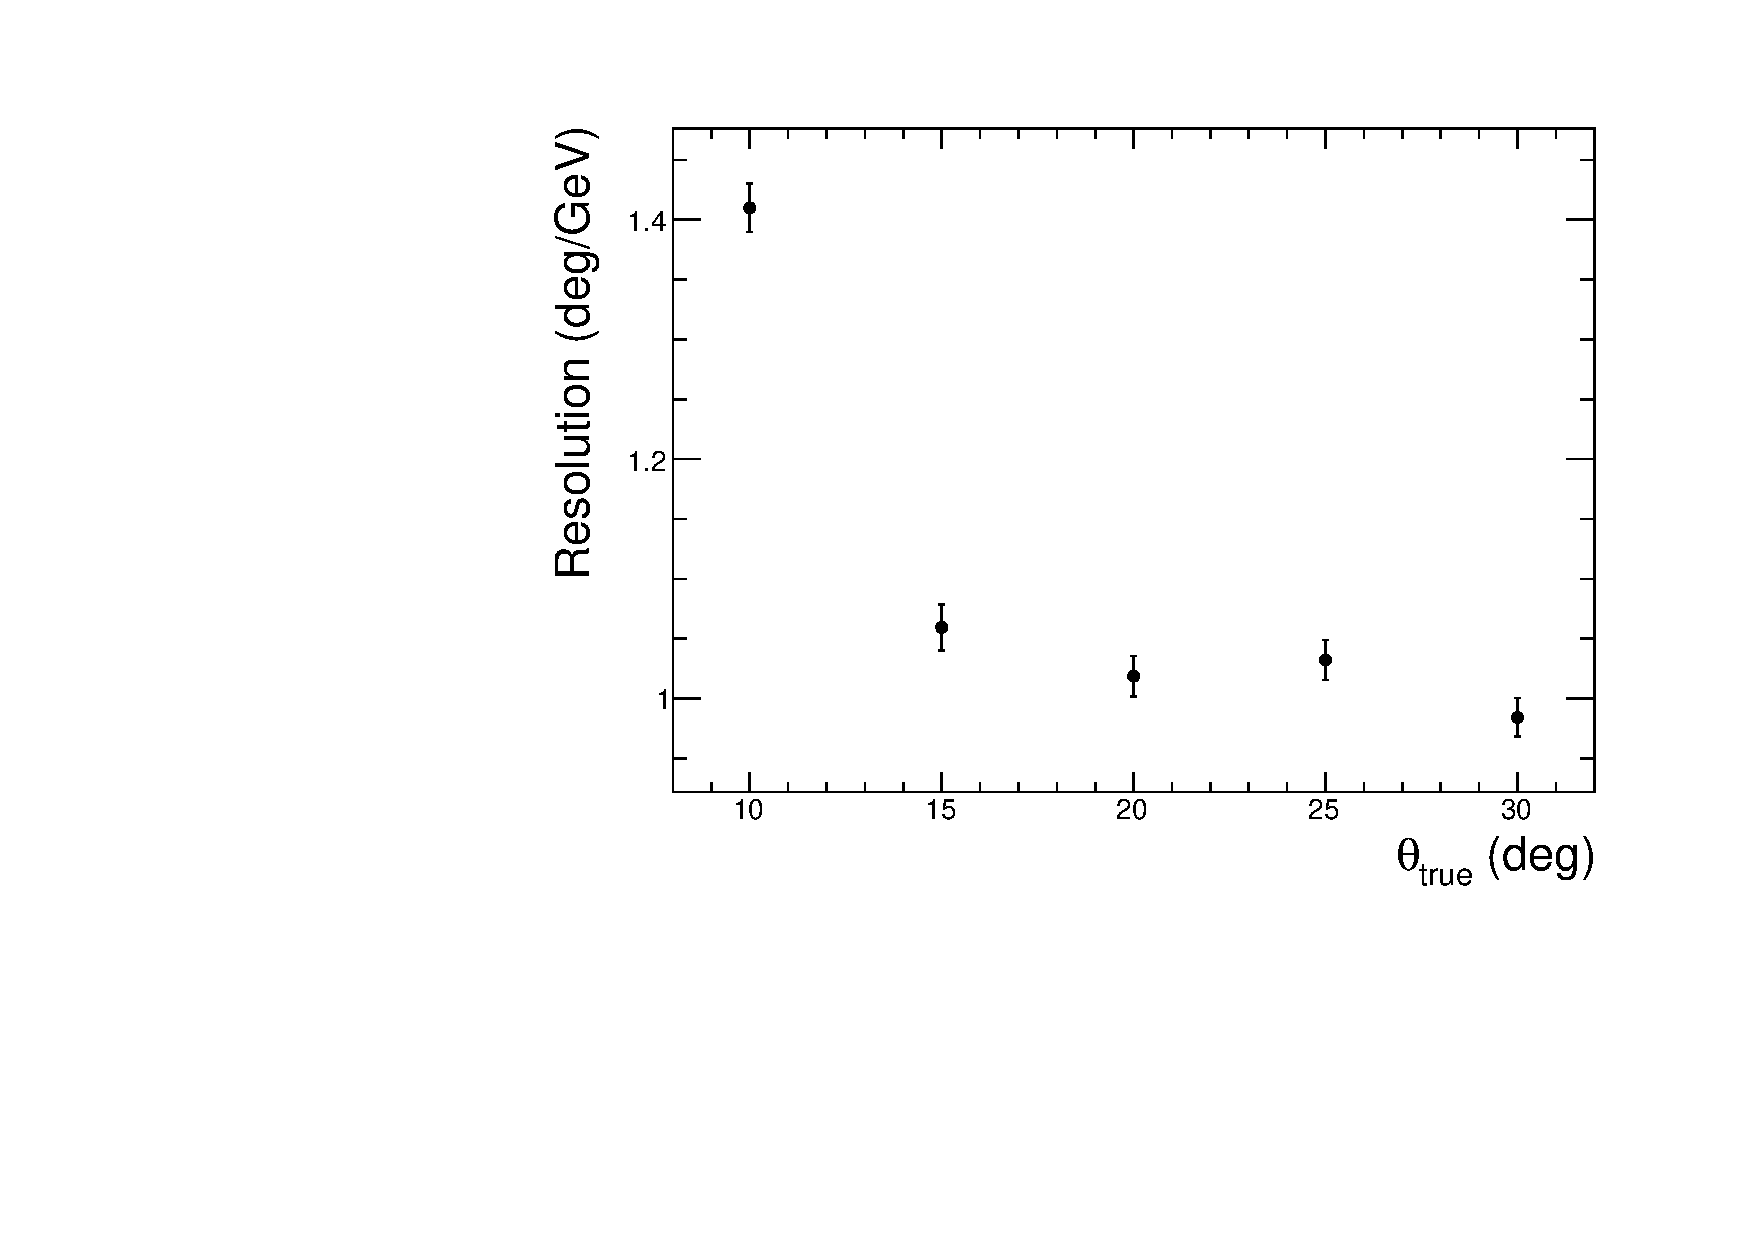
\includegraphics[width=0.48\textwidth]{figures/Fig5_reco_inc.pdf}
}
\DIFaddendFL \caption{ \DIFdelbeginFL \DIFdelFL{The }\DIFdelendFL \DIFaddbeginFL \DIFaddFL{Deduced }\DIFaddendFL angular \DIFdelbeginFL \DIFdelFL{resolution }\DIFdelendFL \DIFaddbeginFL \DIFaddFL{resolutions }\DIFaddendFL as \DIFdelbeginFL \DIFdelFL{a function }\DIFdelendFL \DIFaddbeginFL \DIFaddFL{functions }\DIFaddendFL of \DIFdelbeginFL \DIFdelFL{the $\gamma$ energy }\DIFdelendFL (\DIFdelbeginFL \DIFdelFL{left), and $p_{1}$ for 1 GeV as }\DIFdelendFL a\DIFdelbeginFL \DIFdelFL{function of the incident angle (right}\DIFdelendFL ) \DIFdelbeginFL \DIFdelFL{. $p_{1}$ is consistent down to }\DIFdelendFL \DIFaddbeginFL \DIFaddFL{photon energy for }\DIFaddendFL $\theta=$~\DIFdelbeginFL \DIFdelFL{15~deg }\DIFdelendFL \DIFaddbeginFL \DIFaddFL{10$^{\circ}$ }\DIFaddendFL and \DIFdelbeginFL \DIFdelFL{changing at $\theta=$}\DIFdelendFL \DIFaddbeginFL \DIFaddFL{(b) polar angle for $E_{\gamma}=$}\DIFaddendFL ~\DIFdelbeginFL \DIFdelFL{10}\DIFdelendFL \DIFaddbeginFL \DIFaddFL{1}\DIFaddendFL ~\DIFdelbeginFL \DIFdelFL{deg, which is coming from the definition of $\theta$ }\DIFdelendFL \DIFaddbeginFL \DIFaddFL{GeV. }\DIFaddendFL }
\label{fig:angle_reco_dep_gr}
\end{figure}

Figure~\ref{fig:angle_reco_dep_gr} \DIFaddbegin \DIFadd{(a) }\DIFaddend shows the angular resolution as a function of the incident \DIFdelbegin \DIFdel{$\gamma$ energy }\DIFdelend \DIFaddbegin \DIFadd{photon energy ($E_{\gamma}=$) }\DIFaddend for $\theta=$~10\DIFdelbegin \DIFdel{~degrees on the left panel. The resolution is fitted with $p_{0} + p_{1}/\sqrt{E_{\gamma}(GeV)}$, where the }\DIFdelend \DIFaddbegin \DIFadd{$^{\circ}$. Angular resolutions are fitted with a function of $p_{0} \oplus p_{1}/\sqrt{E_{\gamma}(GeV)}$, where }\DIFaddend $p_{0}$ \DIFdelbegin \DIFdel{denotes the }\DIFdelend \DIFaddbegin \DIFadd{represents an }\DIFaddend energy-independent contribution and is estimated to be \DIFdelbegin \DIFdel{0.2, and the }\DIFdelend \DIFaddbegin \DIFadd{xxx, and }\DIFaddend $p_{1}$ denotes the energy-dependent \DIFdelbegin \DIFdel{contribution}\DIFdelend \DIFaddbegin \DIFadd{parameter}\DIFaddend , mainly related with the development of the EM shower. \DIFdelbegin \DIFdel{The estimated }\DIFdelend $p_{1}$ \DIFdelbegin \DIFdel{for different $\theta$ can be seen on the right panel of fig}\DIFdelend \DIFaddbegin \DIFadd{is estimated to be xxx for $\theta>$~15$^{\circ}$ and xxx$^{\circ}$~$\pm$~xxx$^{\circ}$ for $\theta=$~10$^{\circ}$ in Fig}\DIFaddend .~\ref{fig:angle_reco_dep_gr} \DIFaddbegin \DIFadd{(b). The discrepancy between them is attributed to the followings: polar angle to be always positive and poor angular resolutions for low $E_{\gamma}$ photons. When $\mu$ and $\alpha$ get comparable each other in Eq~\ref{eqn:gg}, the left tail of the distribution would extend to negative area. This largely affects the case $\mu=$~10$^{\circ}$ and not the case $\mu>$~15$^{\circ}$ considering that the angular resolutions for $E_{\gamma}=$~0.1~GeV is estimated to be 4$^{\circ}$}\DIFaddend . 
\DIFdelbegin \DIFdel{They are deviating within $\pm$~0.05~deg range from the 1.1~deg.
}\DIFdelend 

\begin{figure}[!hbt]
\DIFdelbeginFL %DIFDELCMD < 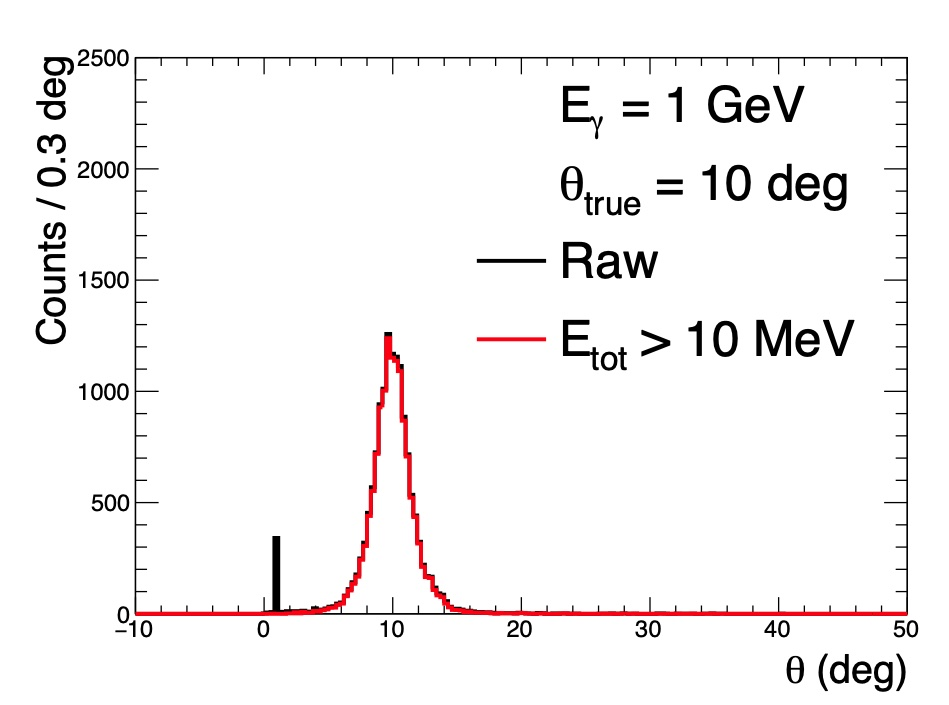
\includegraphics[width=0.48\textwidth]{figures/res_Nlayer.jpg}
%DIFDELCMD < 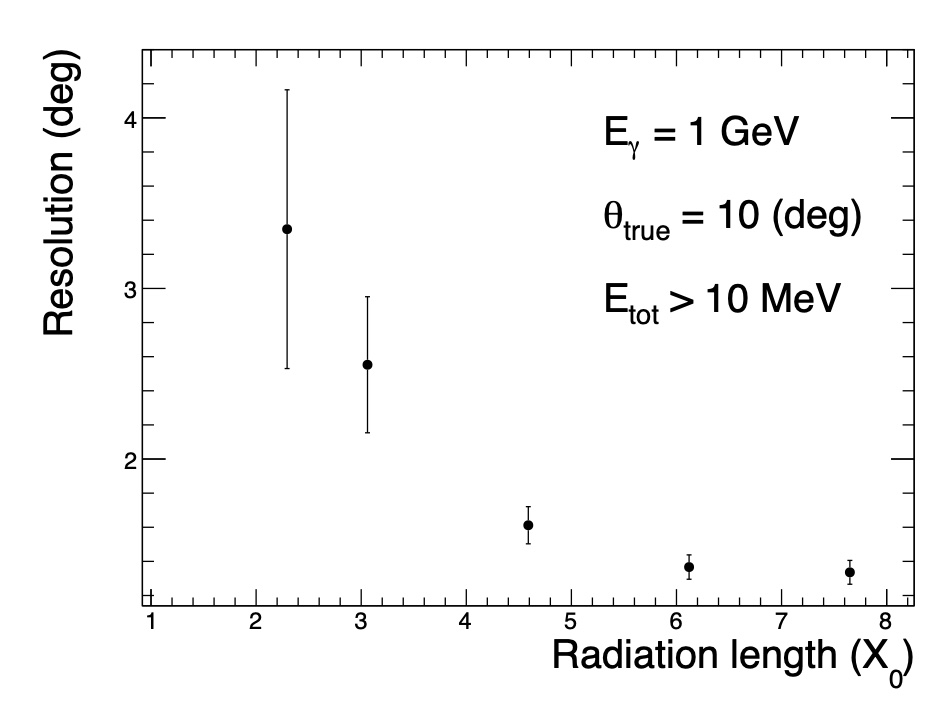
\includegraphics[width=0.48\textwidth]{figures/resol_Nlayer.jpg}
%DIFDELCMD < %%%
\DIFdelendFL \DIFaddbeginFL \stackinset{c}{0.cm}{b}{-0.4cm}{(a)}{
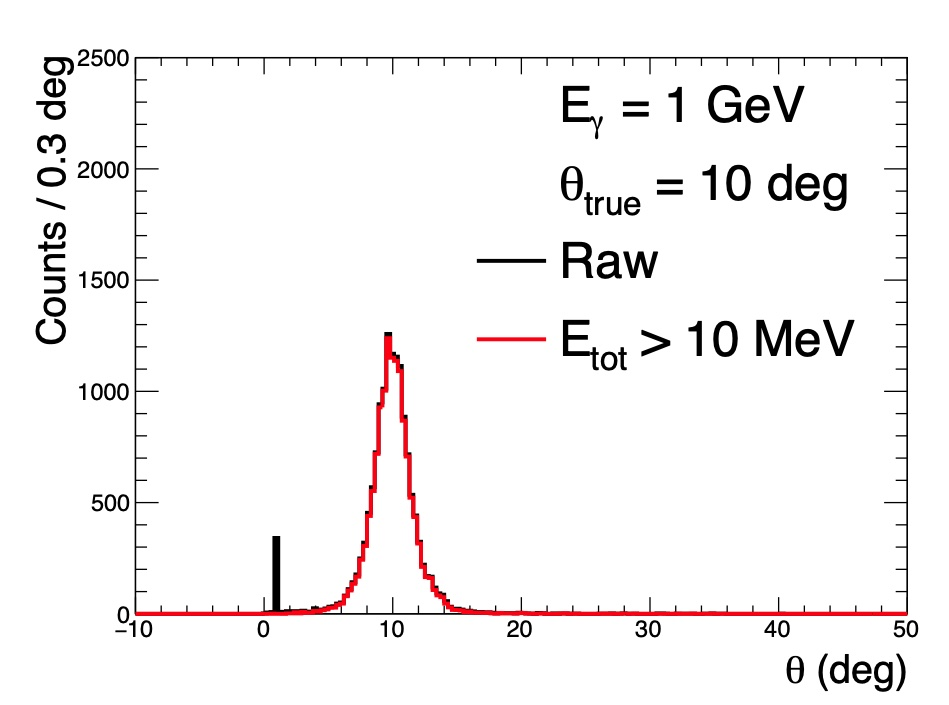
\includegraphics[width=0.48\textwidth]{figures/res_Nlayer.jpg}
}\stackinset{c}{0.cm}{b}{-0.4cm}{(b)}{
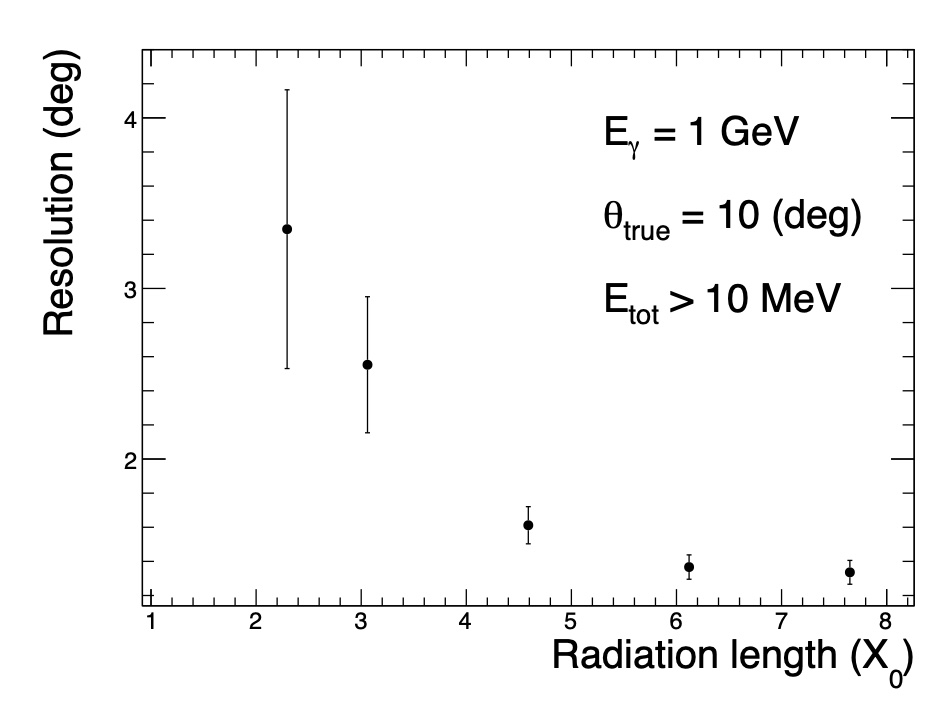
\includegraphics[width=0.48\textwidth]{figures/resol_Nlayer.jpg}
}
\DIFaddendFL \caption{ \DIFaddbeginFL \DIFaddFL{(a) }\DIFaddendFL Reconstructed \DIFaddbeginFL \DIFaddFL{polar angles (}\DIFaddendFL $\theta$\DIFaddbeginFL \DIFaddFL{) }\DIFaddendFL for \DIFdelbeginFL \DIFdelFL{1 GeV $\gamma$ with }\DIFdelendFL \DIFaddbeginFL \DIFaddFL{1-GeV photons at }\DIFaddendFL $\theta=$~10\DIFaddbeginFL \DIFaddFL{$^{\circ}$. Red histogram represents the polar angle distribution by requiring $E_{\rm{tot}}>$}\DIFaddendFL ~\DIFdelbeginFL \DIFdelFL{deg with }\DIFdelendFL \DIFaddbeginFL \DIFaddFL{10~MeV. }\DIFaddendFL (\DIFdelbeginFL \DIFdelFL{red}\DIFdelendFL \DIFaddbeginFL \DIFaddFL{b}\DIFaddendFL ) \DIFdelbeginFL \DIFdelFL{and without (black) the total energy ($E_{\rm{tot}}$) selection (left), and the angular }\DIFdelendFL \DIFaddbeginFL \DIFaddFL{Angular }\DIFaddendFL resolution as a function of \DIFdelbeginFL \DIFdelFL{front layer depth used for the reconstruction }\DIFdelendFL \DIFaddbeginFL \DIFaddFL{radiation length }\DIFaddendFL (\DIFdelbeginFL \DIFdelFL{right}\DIFdelendFL \DIFaddbeginFL \DIFaddFL{$X_{0}$}\DIFaddendFL ).\DIFdelbeginFL \DIFdelFL{The inefficiency for 4.6$X_{0}$ is estimated to be 5.8\% with 10~MeV selection. The large error bars less than 4.6$X_{0}$ is due to insufficient fitting because the reconstructed angular distributions deviated from the General Gaussian function.}\DIFdelendFL }
\label{fig:angle_reco_layer}
\end{figure}

\DIFdelbegin \DIFdel{The reconstruction of the incident angle is tested }\DIFdelend \DIFaddbegin \DIFadd{Furthermore, incidence angles are reconstructed }\DIFaddend with the front \DIFdelbegin \DIFdel{layer instead of the full layers considering the cost-effectiveness from the fact that }\DIFdelend \DIFaddbegin \DIFadd{layers of $X_{0}$ in which }\DIFaddend 99\% of \DIFdelbegin \DIFdel{the $\gamma$ generates the EM shower in front of 5$X_{0}$. The left panel of }\DIFdelend \DIFaddbegin \DIFadd{incident photons generate EM showers. }\DIFaddend Figure~\ref{fig:angle_reco_layer} \DIFdelbegin \DIFdel{shows reconstructed angle using the }\DIFdelend \DIFaddbegin \DIFadd{(a) shows reconstructed angles using }\DIFaddend front 24 layers of the detector, which corresponds to \DIFdelbegin \DIFdel{the }\DIFdelend 4.6$X_{0}$ for \DIFdelbegin \DIFdel{1~GeV $\gamma$. Some $\gamma$s are }\DIFdelend \DIFaddbegin \DIFadd{1-GeV photons. A fraction of photons }\DIFaddend failed to be reconstructed due to the lack of \DIFdelbegin \DIFdel{the channel having the energy deposit}\DIFdelend \DIFaddbegin \DIFadd{active layers}\DIFaddend . The failed events are represented as a delta function near 0, and such events are removed by requiring the total energy deposit to be larger than 10~MeV. The angular resolution with the front layer is estimated to be XXX while possessing inefficiency estimated to be 5.8\%.

\begin{figure}[!hbt]
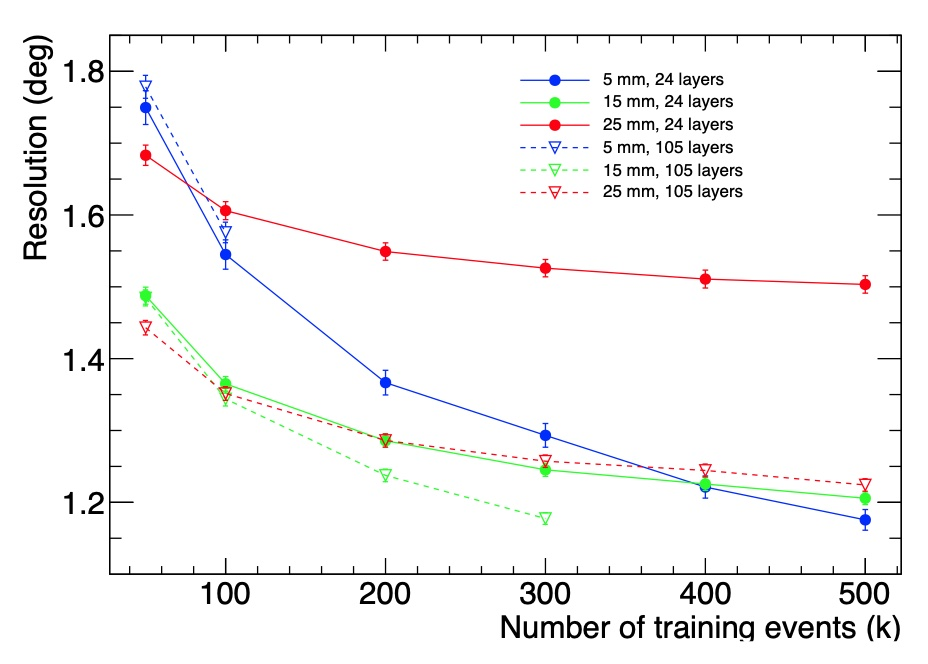
\includegraphics[width=0.6\textwidth]{figures/layer-event.jpg}
\caption{ The angular resolution for \DIFdelbeginFL \DIFdelFL{1 GeV $\gamma$ with }\DIFdelendFL \DIFaddbeginFL \DIFaddFL{1-GeV photons at }\DIFaddendFL $\theta=$~10\DIFdelbeginFL \DIFdelFL{~deg }\DIFdelendFL \DIFaddbeginFL \DIFaddFL{$^{\circ}$ }\DIFaddendFL as a function of the number of training samples with different strip widths using the first 24 layers or the full layers. }
\label{fig:multi-parameter}
\end{figure}

Figure~\ref{fig:multi-parameter} shows the angular resolution with different numbers of training samples for different detector configurations. All configurations show a decrease in the angular resolution with increasing training samples, which means that enhanced statistics for the training results in better reconstruction. The angular resolution with 5-mm-wide scintillator strips \DIFdelbegin \DIFdel{is more rapidly decreasing }\DIFdelend \DIFaddbegin \DIFadd{decreases more rapidly }\DIFaddend than others. The number of features for the 5-mm-wide strip is much larger than others, and the number of training samples is much required to correlate larger features. Considering limited computing resources, \DIFdelbegin \DIFdel{The setup with 2$\times10^{5}$ }\DIFdelend \DIFaddbegin \DIFadd{the setup with $10^{5}$ }\DIFaddend events, 24 layers, and the 15-mm-wide strip \DIFdelbegin \DIFdel{is chosen for the training of }\DIFdelend \DIFaddbegin \DIFadd{was chosen for training }\DIFaddend the $\XGB$ \DIFdelbegin \DIFdel{, where the result is under }\DIFdelend \DIFaddbegin \DIFadd{model. The training result differs by only }\DIFaddend 0.1\DIFdelbegin \DIFdel{degree difference }\DIFdelend \DIFaddbegin \DIFadd{$^{\circ}$ }\DIFaddend from the best setup \DIFaddbegin \DIFadd{will full layers}\DIFaddend .

\section{SUMMARY}
\label{sec:sum}

We \DIFdelbegin \DIFdel{conduct a feasibility study to measure the incident angle of the $\gamma$ with the finely segmented sampling calorimeter. With alternating 1-mm-thick lead plates and 5-mm-thick plastic scintillator strips, the EM shower is largely generated in lead sheets, and is measured by scintillators.The incident angle the $\gamma$ is reconstructed with the }\DIFdelend \DIFaddbegin \DIFadd{report simulation results on the incidece angle reconstruction of EM sampling calorimeters with photons being in the range of 100~MeV to 2~GeV. EM shwers are simulated in the new samplinng calorimeter.using Geant4. We utilize the }\DIFaddend $\XGB$ \DIFdelbegin \DIFdel{using the energy deposited in each scintillator strip }\DIFdelend \DIFaddbegin \DIFadd{model to reconstruct the photon incident angle by correlating all energy deposits in each strip with the incidence angle all events together}\DIFaddend .

We \DIFdelbegin \DIFdel{optimize }\DIFdelend \DIFaddbegin \DIFadd{tune }\DIFaddend the hyperparameter of the $\XGB$ \DIFdelbegin \DIFdel{, and optimize the detector configuration using the optimized $\XGB$. We scan the hyperparameter in the 5-dimensional space and find the set providing the best angular resolution for different detector configurations}\DIFdelend \DIFaddbegin \DIFadd{to reconstruct the incidence angle with the best angular resolution, and study the angular resolution in terms of the detector configuration}\DIFaddend . We find that 15-mm-wide strips provide the best angular resolution, which can be expressed as 0.2\DIFdelbegin \DIFdel{+}\DIFdelend \DIFaddbegin \DIFadd{~$\oplus~$}\DIFaddend 1.1\DIFdelbegin \DIFdel{$/ \sqrt{E_\gamma}$ }\DIFdelend \DIFaddbegin \DIFadd{$/\sqrt{E_\gamma}$ }\DIFaddend for different incident angles. We also \DIFdelbegin \DIFdel{find }\DIFdelend \DIFaddbegin \DIFadd{conclude }\DIFaddend that using 24 front layers gives the angular resolution which is \DIFdelbegin \DIFdel{compatible }\DIFdelend \DIFaddbegin \DIFadd{comparable }\DIFaddend with the angular resolution we get from the full layer.

\DIFdelbegin \DIFdel{The }\DIFdelend \DIFaddbegin \DIFadd{We study that the }\DIFaddend angular resolution is changing with the variation of the training of the $\XGB$ and the detector configuration. As the strip width decreases, more channels of scintillator strips are required, and the training of the $\XGB$ gets affected due to the increased feature size. This is quenched with the larger number of training samples, which qualitatively improves the training of the $\XGB$. On the other hand, the longer strip width provides the worse angular resolution as the position resolution of the EM shower gets worse. We conclude that 15-mm-wide strips provide the favorable angular resolution with 24 front layers and \DIFdelbegin \DIFdel{2$\times10^{5}$ }\DIFdelend \DIFaddbegin \DIFadd{$10^{5}$ }\DIFaddend training samples.

\label{sec:con}


%\pagebreak

\begin{acknowledgments}
\end{acknowledgments}

\bibliography{paper}

\end{document}
